%%%%%%%%%%%%%%%%%%%%%%%%%%%%%%%%%%%%%%%%%%%%%%%%%%%%%%%%%%%%%%%%%%%%%%%%%%%%%%%%%%%%%%
% To make formatting easy tell LaTeX what kind of document you want to write
% by changing the according {} to {#1}
%%%%%%%%%%%%%%%%%%%%%%%%%%%%%%%%%%%%%%%%%%%%%%%%%%%%%%%%%%%%%%%%%%%%%%%%%%%%%%%%%%%%%%
%
% Most of the choices and things that need to be adjusted are maked 
% with a commented "TODO". Adjust the given value the one correct your your case.
%
%%%%%%%%%%%%%%%%%%%%%%%%%%%%%%%%%%%%%%%%%%%%%%%%%%%%%%%%%%%%%%%%%%%%%%%%%%%%%%%%%%%%%%

% Dissertation
\newcommand{\Diss}[1]{}
% Diplomarbeit
\newcommand{\Dipl}[1]{}
% Master Thesis
\newcommand{\MS}[1]{#1}
% Studienarbeit
\newcommand{\Stud}[1]{}

\newcommand{\BachelorT}[1]{} %%TODO: mark the corret one with a #1

%%%%%%%%%%%%%%%%%%%%%%%%%%%%%%%%%%%%%%%%%%%%%%%%%%%%%%%%%%%%%%%%%%%%%%%%%%%%%%%%%%%%%%
% Which language do you want to write in
%%%%%%%%%%%%%%%%%%%%%%%%%%%%%%%%%%%%%%%%%%%%%%%%%%%%%%%%%%%%%%%%%%%%%%%%%%%%%%%%%%%%%%
%English
\newcommand{\EN}[1]{#1} %%TODO: Choose the correct language
%German
\newcommand{\DE}[1]{}

%%%%%%%%%%%%%%%%%%%%%%%%%%%%%%%%%%%%%%%%%%%%%%%%%%%%%%%%%%%%%%%%%%%%%%%%%%%%%%%%%%%%%%
% For print single or double page?
%%%%%%%%%%%%%%%%%%%%%%%%%%%%%%%%%%%%%%%%%%%%%%%%%%%%%%%%%%%%%%%%%%%%%%%%%%%%%%%%%%%%%%
\newcommand{\single}[1]{#1} %%TODO: Choose
\newcommand{\double}[1]{}

%%%%%%%%%%%%%%%%%%%%%%%%%%%%%%%%%%%%%%%%%%%%%%%%%%%%%%%%%%%%%%%%%%%%%%%%%%%%%%%%%%%%%%
% Now this is followed by a lot of page and command definitions. For the beginning you 
% should be able to continue where you find the next comment section like this one.
% However, you might want to take a look a the definitions sometime to be able to use 
% them. Of course you can also add the defintions you needed yourself.
%%%%%%%%%%%%%%%%%%%%%%%%%%%%%%%%%%%%%%%%%%%%%%%%%%%%%%%%%%%%%%%%%%%%%%%%%%%%%%%%%%%%%%

\single{\documentclass[12pt,a4paper,oneside,german,english,fleqn]{book}}
\double{\documentclass[12pt,a4paper,twoside,german,english,fleqn]{book}}
\usepackage[normalem]{ulem}
\usepackage[ngerman,main=english]{babel}
%\usepackage[draft,breaklinks=true,colorlinks=false,dvips,bookmarks,pdffitwindow,pdfcenterwindow=true,pdfstartview=Fit]{hyperref}
%\usepackage[breaklinks=true,colorlinks=false,dvips,bookmarks,pdffitwindow,pdfcenterwindow=true,pdfstartview=Fit]{hyperref}
\usepackage{setspace}
\usepackage{cite}
\usepackage{float,times} 
\usepackage[utf8x]{inputenc}
\usepackage[T1]{fontenc}
\usepackage{amsmath,amsthm,latexsym,amssymb}
\usepackage[dvips]{epsfig}
% \usepackage{subfigure}
\usepackage{rotating}

\usepackage{graphicx}
\usepackage{subcaption}

%\usepackage[outputdir=obj/]{minted} %% Use for advanced build mechanic, needs newest minted style file
%\usepackage{minted} %% use for fancy syntax highlighting of code. Needs "pygmetize" and the minted style file
\usepackage{xspace}

\usepackage{xcolor}
\usepackage{afterpage}
\usepackage{multirow}
\usepackage{array}

\usepackage{pdfpages}

\usepackage{booktabs}% http://ctan.org/pkg/booktabs
\newcommand{\tabitem}{~~\llap{\textbullet}~~}

\usepackage{capt-of}
\usepackage{caption}
\usepackage{listings}
% \renewcommand{\lstlistingname}{Quelltext}
\renewcommand*{\lstlistlistingname}{List of \lstlistingname s}
%\usepackage[german]{fancyref}
\usepackage[english]{fancyref}
\newcommand*{\fancyreflstlabelprefix}{lst}
\newcommand*{\fancyrefitelabelprefix}{ite}
\newcommand*{\fancyrefparlabelprefix}{par}

\fancyrefaddcaptions{german}{
  \providecommand*{\freflstname}{Listing}
  \providecommand*{\Freflstname}{Listing}
}

\frefformat{plain}{\fancyreflstlabelprefix}{\freflstname\fancyrefdefaultspacing#1}
\Frefformat{plain}{\fancyreflstlabelprefix}{\Freflstname\fancyrefdefaultspacing#1}

\frefformat{plain}{\fancyreflstlabelprefix}{
  \freflstname\fancyrefdefaultspacing#1#3
}
\Frefformat{plain}{\fancyreflstlabelprefix}{
  \Freflstname\fancyrefdefaultspacing#1#3
}

\fancyrefaddcaptions{german}{
  \providecommand*{\frefitename}{Liste}
  \providecommand*{\Frefitename}{Liste}
}

\frefformat{plain}{\fancyrefitelabelprefix}{\frefitename\fancyrefdefaultspacing#1}
\Frefformat{plain}{\fancyrefitelabelprefix}{\Frefitename\fancyrefdefaultspacing#1}

\frefformat{plain}{\fancyrefitelabelprefix}{
  \frefitename\fancyrefdefaultspacing#1#3
}
\Frefformat{plain}{\fancyrefitelabelprefix}{
  \Frefitename\fancyrefdefaultspacing#1#3
}

\fancyrefaddcaptions{german}{
  \providecommand*{\frefparname}{Paragraph}
  \providecommand*{\Frefparname}{Paragraph}
}

\frefformat{plain}{\fancyrefparlabelprefix}{\frefparname\fancyrefdefaultspacing#1}
\Frefformat{plain}{\fancyrefparlabelprefix}{\Frefparname\fancyrefdefaultspacing#1}

\frefformat{plain}{\fancyrefparlabelprefix}{
  \frefparname\fancyrefdefaultspacing#1#3
}
\Frefformat{plain}{\fancyrefparlabelprefix}{
  \Frefparname\fancyrefdefaultspacing#1#3
}

\renewcommand{\fancyrefdefaultformat}{plain}

\newcommand{\ThesisTitle}{Property Generation for Pipelined Processors in a Property-Driven Design Approach} %%TODO
\newcommand{\ThesisTitleGerman}{Hier Deutschen Titel Einf\"ugen} %%TODO %NOTE: for some reason, LaTeX does not understand utf8 here...

% format page layout.

%\setlength{\topmargin}{0cm}
%\setlength{\textwidth}{15cm}
%\setlength{\textheight}{22cm}
%\setlength{\oddsidemargin}{1cm}
%\setlength{\evensidemargin}{0cm}
\setlength{\headheight}{15pt}

\setlength{\emergencystretch}{1em}

\setlength{\voffset}{-0cm}
\setlength{\topmargin}{0cm}
\setlength{\headheight}{0.54cm}
\setlength{\textheight}{23cm}
% \setlength{\headsep}{1.5cm}
% \setlength{\hoffset}{-2.54cm}
\setlength{\hoffset}{0cm}
\setlength{\oddsidemargin}{0.46cm}
\setlength{\evensidemargin}{0.46cm}
\setlength{\textwidth}{15cm}
\setlength{\marginparsep}{0cm}
\setlength{\marginparwidth}{1.54cm}

% adjust linespacing
\linespread{1.3}

\usepackage{parskip}
% \setlength{\footskip}{1cm}
% \setlength{\parindent}{0cm}
 \setlength{\parskip}{1em}

\setcounter{secnumdepth}{3}
\setcounter{tocdepth}{1}

\usepackage{fancyhdr}
\pagestyle{fancy}
\fancyhead{} % clear all header fields
\double{\fancyhead[LE]{\slshape \nouppercase{\leftmark}}} % chapter titles
\fancyhead[RO]{\slshape \nouppercase{\rightmark}} % section titles
\fancyfoot{} % clear all footer fields
\fancyfoot[C]{\thepage}


\usepackage[%dvips,
	colorlinks=false,
	bookmarks,
	pdffitwindow,
	pdfcenterwindow=true,
	pdfstartview=Fitpdftex,
	pdfauthor={Insert Author Name here}, %%TODO
% 	pdftitle={\EN{\ThesisTitle}\DE{\ThesisTitleGerman}},
	pdftitle={\EN{\ThesisTitle}},
	pdfsubject={}, % one sentence summery %%TODO
	pdfkeywords={Thesis,Hardware,Simulation,System-Modelling}, %TODO: comma-seperated keywords
	pdfproducer={Latex with hyperref},
	pdfcreator={}]{hyperref}

%%%%%%%%%%%%%%%%%%%%%%%%%%%%%%%%%%%%%%%%%%%%%%%%%%%
% Overly fancy comments
%%%%%%%%%%%%%%%%%%%%%%%%%%%%%%%%%%%%%%%%%%%%%%%%%%%
%% uncomment the ifthen block if the enhanched build mechanic is used
% \providecommand\printcomments{false}
% \usepackage{ifthen}
% \ifthenelse{ \equal{\printcomments}{true} }{
\newcommand{\comment}[3]{\marginpar{\textcolor{#2}{Comment: #1}}\textcolor{#2}{\textit{[#1: #3]}}}
\newcommand{\SupervisorComment}[1]{\comment{Supervisor}{red}{#1}} %%TODO: exchange "SupervisorComment" and "Supervisor" with initials
\newcommand{\StudentComment}[1]{\comment{Student}{blue}{#1}} %%TODO: exchange "StudentComment" and "Student" with initials
% }{
% \newcommand{\TF}[1]{}
% \newcommand{\LA}[1]{}
% }
%%%%%%%%%%%%%%%%%%%%%%%%%%%%%%%%%%%%%%%%%%%%%%%%%%%
%\usepackage{showframe}

\usepackage[shortlabels]{enumitem}

%%%%%%%%%%%%%%%%%%%%%%%%%%%%%%%%%%%%%%%%%%%%%%%%%%%%%%%%%%%%%%%%%%%%%%%%%%%%%%
% 
%  Some useful definitions 
% 
%%%%%%%%%%%%%%%%%%%%%%%%%%%%%%%%%%%%%%%%%%%%%%%%%%%%%%%%%%%%%%%%%%%%%%%%%%%%%%


\newcommand{\refsec}[1]{Sec.~\ref{sec:#1}}
\newcommand{\reffig}[1]{Fig.~\ref{fig:#1}}
\newcommand{\reftab}[1]{Tab.~\ref{tab:#1}}
\newcommand{\refalg}[1]{Alg.~\ref{alg:#1}}
\newcommand{\refdef}[1]{Def.~\ref{def:#1}}

\newcommand{\URLFORMAT}[1]{\mbox{\sffamily\small #1}}

\newcommand{\CODESYMBOL}[1]{\textsf{\textit{\small #1}}}

\newcommand{\CTLOPERATOR}[1]{\mbox{\textsf{\textup{#1}}}}
\newcommand{\CTLAX}{\CTLOPERATOR{AX}}
\newcommand{\CTLAF}{\CTLOPERATOR{AF}}
\newcommand{\CTLAG}{\CTLOPERATOR{AG}}
\newcommand{\CTLEX}{\CTLOPERATOR{EX}}
\newcommand{\CTLEF}{\CTLOPERATOR{EF}}
\newcommand{\CTLEG}{\CTLOPERATOR{EG}}
\newcommand{\LTLX}{\CTLOPERATOR{X}}
\newcommand{\LTLXT}[1]{\mbox{$\CTLOPERATOR{X}^{#1}$}}
\newcommand{\LTLF}{\CTLOPERATOR{F}}
\newcommand{\LTLG}{\CTLOPERATOR{G}}
\newcommand{\LTLU}{\CTLOPERATOR{U}}
\newcommand{\LTLR}{\CTLOPERATOR{R}}
\newcommand{\LTLW}{\CTLOPERATOR{W}}

\newcommand{\LTLS}{\CTLOPERATOR{S}}



%%%%%%%%%%%%%%%%%%%%%%%%%%%%%%%%%%%%%%%%%%%%%%%%%%%%%%%%%%%%%%%%%%%%%%%%%%%%%%
% For revisions: 
\definecolor{newtextcolor}{rgb}{0,0,0.5}
\newenvironment{newtext}{\color{newtextcolor}}{}
\definecolor{oldtextcolor}{rgb}{0.4,0.4,0.4}
\newenvironment{oldtext}{\color{oldtextcolor}\par\textit{\sffamily Begin (old
    text)}\par}{\hfill\textit{\sffamily End (old text)}\par}
\newcommand{\textnew}[1]{{\color{newtextcolor}#1}}


%For code: 
\newcommand{\key}[1]{\textcolor{BlueViolet}{#1}}
\newcommand{\ckey}[1]{\textcolor{blue}{#1}}
\newcommand{\type}[1]{\textcolor{Green}{#1}}
\newcommand{\port}[1]{\textcolor{RedViolet}{#1}}
\newcommand{\macro}[1]{\textcolor{Sepia}{#1}}
\newcommand{\tend}{\key{t\_end}\textcolor{RedViolet}{(}length\textcolor{RedViolet}{)}~\textcolor{RedViolet}{\#\#}0~}
\newcommand{\tstart}{ \key{t} \textcolor{RedViolet}{\#\#}0~}

%ITL Properties:
\newcommand{\ITLKW}[1]{{\color{blue} #1}}
\newcommand{\ITLAT}[1]{\ITLKW{at t+{}#1: }}
\newcommand{\ITLOR}{\ITLKW{\textbar\,\textbar}}
\newcommand{\ITLENDL}{\ITLKW{;}}
\newcommand{\ITLPREV}{\ITLKW{prev}}
\definecolor{DARKGREEN}{RGB}{0,100,0}
\newcommand{\ITLCOMMENT}[1]{{\color{DARKGREEN}- - #1}}


%Text

\newcommand{\tsCODE}[1]{\textsf{\textit{\small #1}}}

%Environments
\newtheorem{definition}{Definition}
\newtheorem{theorem}{Theorem}

%Abbreviations:
\newcommand{\SYSTEMCPPA}{SystemC-PPA}
\newcommand{\NOP}{non-overlap pipelining}
\newcommand{\OP}{overlap pipelining}
\newcommand{\BP}{base property}
\newcommand{\RP}{relaxed property}
\newcommand{\PPDD}{PPDD}
\newcommand{\PDDTOOL}{DeSCAM} 
\newcommand{\SYMBOLNAME}[1]{\mbox{\textsf{\textsl{\small #1}}\,}}
\newcommand{\BOOLTRUE}{\SYMBOLNAME{true}} 
\newcommand{\BOOLFALSE}{\SYMBOLNAME{false}}

% symbols of PPA
\newcommand{\CONCAT}{\mbox{$\odot$}}
\newcommand{\IMPORTANT}{\mbox{$\Psi$}}
  % message predicate
\newcommand{\MSGPRED}{\mbox{$\mu$}}
  % operational input predicate
\newcommand{\INPPRED}{\mbox{$\iota$}}
  % trigger 
\newcommand{\TRIGPRED}{\mbox{$\iota$}}

  %operational path
\newcommand{\oppath}{\ensuremath\mbox{$\mathtt{opath}$}}
%\newcommand\oppath{\mathrel{\overset{\makebox[0pt]{\mbox{\normalfont\tiny\sffamily oper}}}{\pi}}}

  %operational output
%\newcommand{\opout}{\ensuremath\mbox{$\mathtt{oout}$}}

  %color similar symbol
\newcommand\colsim{\mathrel{\overset{\makebox[0pt]{\mbox{\normalfont\tiny\sffamily color}}}{=}}}

%state, input, output color
\newcommand{\nodecolor}{\ensuremath\mbox{$\mathtt{f_{C}}$}}
\newcommand{\statecolor}{\ensuremath\mbox{$\mathtt{f_{SC}}$}}
\newcommand{\incolor}{\ensuremath\mbox{$\mathtt{f_{XC}}$}}
\newcommand{\outcolor}{\ensuremath\mbox{$\mathtt{f_{YC}}$}}

\newcommand{\notimplies}{%
  \mathrel{{\ooalign{\hidewidth$\not\phantom{=}$\hidewidth\cr$\implies$}}}}


% PredCol
\newcommand{\statepredcolor}{\ensuremath\mbox{$\mathtt{B_{\eta{}C}}$}}
\newcommand{\inputpredcolor}{\ensuremath\mbox{$\mathtt{B_{\iota{}C}}$}}
\newcommand{\outputpredcolor}{\ensuremath\mbox{$\mathtt{B_{\mu{}C}}$}}
% ColPred
\newcommand{\statecolorpred}{\ensuremath\mbox{$\mathtt{B_{C\eta}}$}}
\newcommand{\inputcolorpred}{\ensuremath\mbox{$\mathtt{B_{C\iota}}$}}
\newcommand{\outputcolorpred}{\ensuremath\mbox{$\mathtt{B_{C\mu}}$}}


% text style for operators: 
\newcommand{\tsOPERATOR}[1]{\mbox{\textrm{\textup{#1}}}}

% IMG and other operators
\newcommand{\IMG}{\tsOPERATOR{img}} %image
\newcommand{\PRE}{\tsOPERATOR{pre}} %pre-image

\newcommand\LFP{\mathrel{\overset{\makebox[0pt]{\mbox{\normalfont\scriptsize\sffamily fp}}}{\mbox{\normalfont\footnotesize\sffamily <}}}}
\newcommand\GFP{\mathrel{\overset{\makebox[0pt]{\mbox{\normalfont\scriptsize\sffamily fp}}}{\mbox{\normalfont\footnotesize\sffamily >}}}}

\newcommand{\ISPATH}{\tsOPERATOR{ispath}}
\newcommand{\ISOPERATION}{\tsOPERATOR{isoperation}}
\newcommand{\ISOUTPUT}{\tsOPERATOR{isoutput}}
\newcommand{\INPUT}{\tsOPERATOR{input}}
\newcommand{\OUTPUT}{\tsOPERATOR{output}}
% \newcommand{\ANY}{\tsOPERATOR{any}}
\newcommand{\STUTTER}{\tsOPERATOR{stutter}}

% NEXT operator takes a subscript in math mode: 
\newcommand{\NEXT}[1]{\mbox{\tsOPERATOR{next}}_{#1}}


%%% Local Variables: 
%%% mode: latex
%%% TeX-master: "binder"
%%% End: 


%%%%%%%%%%%%%%%%%%%%%%%%%%%%%%%%%%%%%%%%%%%%%%%%%%%%%%%%%%%%%%%%%%%%%%%%%%%%%%
%  Collaborative editing in EIS group
%  
%  Let NN be your initials. 
%  The following macros are defined: 
%
%  \NNINS{a}     - Suggest inserting the text a. 
%  \NNDEL{a}     - Suggest deleting the text a. 
%  \NNREP{a}{b}  - Suggest replacing a by b. 
%  \NNSAY{a}     - Comment by saying a.
% 
%%%%%%%%%%%%%%%%%%%%%%%%%%%%%%%%%%%%%%%%%%%%%%%%%%%%%%%%%%%%%%%%%%%%%%%%%%%%%%


%%%%%%%%%%%%%%%%%%%%%%%%%%%%%%%%%%%%%%%%%%%%%%%%%%%%%%%%%%%%%%%%%%%%%%%%%%%%%%
%
%   Required packages:
% 
%   \usepackage{xcolor}
%   \usepackage{ifthen}
%   \usepackage[normalem]{ulem}
%
%   Place those in the file prefix.tex
%
%%%%%%%%%%%%%%%%%%%%%%%%%%%%%%%%%%%%%%%%%%%%%%%%%%%%%%%%%%%%%%%%%%%%%%%%%%%%%%


%%%%%%%%%%%%%%%%%%%%%%%%%%%%%%%%%%%%%%%%%%%%%%%%%%%%%%%%%%%%%%%%%%%%%%%%%%%%%%
% MARKUP switch
% Set to true if markup is to be shown, false otherwise

\newboolean{MARKUP}
\setboolean{MARKUP}{true}
% \setboolean{MARKUP}{false}

%
%%%%%%%%%%%%%%%%%%%%%%%%%%%%%%%%%%%%%%%%%%%%%%%%%%%%%%%%%%%%%%%%%%%%%%%%%%%%%%

%%%%%%%%%%%%%%%%%%%%%%%%%%%%%%%%%%%%%%%%%%%%%%%%%%%%%%%%%%%%%%%%%%%%%%%%%%%%%%
%
%  Authors

%  Every author can have their own distinctive markup color. 

%  WK - Wolfgang Kunz
\definecolor{ColorWK}{rgb}{0.8,0,0}
%  DS - Dominik Stoffel
\definecolor{ColorDS}{rgb}{0, 0, 1.0}

%  AD - Anna Lena Duque Anton
\definecolor{ColorAD}{rgb}{0.7,0.7,0.7}
%  AK - Ammar Ben Khadra
\definecolor{ColorAK}{rgb}{0.7,0.7,0.7}
%  CB - Christian Bartsch
\definecolor{ColorCB}{rgb}{0.7,0.7,0.7}
%  JM - Johannes Mueller
\definecolor{ColorJM}{rgb}{0.7,0.7,0.7}
%  JU - Joakim Urdahl
\definecolor{ColorJU}{rgb}{0,0.5,0}
%  KD - Keerthikumara Devarajegowda 
\definecolor{ColorKD}{rgb}{0.1,0.6,0.3}
%  MF - Mohammad Fadiheh
\definecolor{ColorMF}{RGB}{0,126,0}
%  MS - Michael Schwarz
\definecolor{ColorMS}{RGB}{255,140,0}
%  PM - Paulius Morkunas
\definecolor{ColorPM}{rgb}{0.0, 0.47, 0.75}
%  SS - Stian Sorensen
\definecolor{ColorSS}{RGB}{192,88,0}
%  SU - Shrinidhi Udupi
\definecolor{ColorSU}{rgb}{0.1,0.5,0.5}
%  TF - Thomas Fehmel
\definecolor{ColorTF}{RGB}{192,88,0}
\definecolor{ColorTFX}{RGB}{152,48,0}
%  TL - Tobias Ludwig
\definecolor{ColorTL}{RGB}{33,190,190}

\definecolor{ColorNN}{rgb}{0.9,0.0,0.0}


% pretty green
\definecolor{ColorINSERT}{RGB}{0, 192, 0}
% pretty gray
\definecolor{ColorDELETE}{RGB}{108,108,108}

\newcommand{\PRINTCOLORLIST}{%
\par\textcolor{ColorWK}{Wolfgang Kunz}%
\par\textcolor{ColorDS}{Dominik Stoffel}%
\par\textcolor{ColorAD}{Anna Lena Duque Ant\'{o}n}%
\par\textcolor{ColorAK}{Ammar Ben Khadra}%
\par\textcolor{ColorCB}{Christian Bartsch}%
\par\textcolor{ColorJU}{Joakim Urdahl}%
\par\textcolor{ColorKD}{Keerthikumara Devarajegowda}%
\par\textcolor{ColorJM}{Johannes M\"uller}%
\par\textcolor{ColorMF}{Mohammad Fadiheh}%
\par\textcolor{ColorMS}{Michael Schwarz}%
\par\textcolor{ColorPM}{Paulius Morku\~{n}as}%
\par\textcolor{ColorSU}{Shrinidhi Udupi}%
\par\textcolor{ColorSS}{Stian S\o rensen}%
\par\textcolor{ColorTF}{Thomas Fehmel}%
\par\textcolor{ColorTL}{Tobias Ludwig}%
}%

%
%%%%%%%%%%%%%%%%%%%%%%%%%%%%%%%%%%%%%%%%%%%%%%%%%%%%%%%%%%%%%%%%%%%%%%%%%%%%%%


%%%%%%%%%%%%%%%%%%%%%%%%%%%%%%%%%%%%%%%%%%%%%%%%%%%%%%%%%%%%%%%%%%%%%%%%%%%%%%
% Macro definitions

% The macro \sout is from the ulem package. 
% \usepackage[normalem]{ulem}
\newcommand{\STRIKETHROUGH}[1]{\sout{#1}}


\newcommand{\tsSAY}[1]{\slshape\sffamily\color{#1}}
\newcommand{\tsINITIALS}[2]{\color{#1}\raisebox{0.7ex}{\tiny\bfseries #2}}
\newcommand{\tsWON}[2]{\color{#1}\sffamily\raisebox{0.2ex}{\footnotesize\itshape #2}}
% highlighting for the EISCOM markup
\newcommand{\tsHL}[1]{\hl{#1}}
% \newcommand{\tsHL}[1]{\colorbox{yellow}{#1}}

% commands
\newcommand{\EISREP}[4]{{\ifthenelse{\boolean{MARKUP}}{\tsINITIALS{#2}{(#1)}\,\STRIKETHROUGH{#3}\hspace{0.4ex}{{#4}}}{{#4}}}}
\newcommand{\EISDEL}[3]{{\ifthenelse{\boolean{MARKUP}}{\tsINITIALS{#2}{(#1)}\,\STRIKETHROUGH{#3}\hspace{0.4ex}}{}}}
\newcommand{\EISINS}[3]{{\ifthenelse{\boolean{MARKUP}}{\tsINITIALS{#2}{(#1)}\,{#3}}{{#3}}}}
% accepted version
\newcommand{\aEISREP}[4]{{\ifthenelse{\boolean{MARKUP}}{{\color{ColorINSERT}{#4}}}{{#4}}}}
\newcommand{\aEISDEL}[3]{{\ifthenelse{\boolean{MARKUP}}{{\color{red}$\wr\wr$}}{}}}
\newcommand{\aEISINS}[3]{{\ifthenelse{\boolean{MARKUP}}{{\color{ColorINSERT}{#3}}}{#3}}}
% rejected version
\newcommand{\rEISREP}[4]{{\ifthenelse{\boolean{MARKUP}}{\tsINITIALS{(#2)}{\STRIKETHROUGH{#1}~KEEP:}\,\uline{#3}{\color{ColorDELETE}\STRIKETHROUGH{#4}}}{{#3}}}}
\newcommand{\rEISDEL}[3]{{\ifthenelse{\boolean{MARKUP}}{\tsINITIALS{(#2)}{\STRIKETHROUGH{#1}~KEEP:}\,\uline{#3}}{{#3}}}}
\newcommand{\rEISINS}[3]{{\ifthenelse{\boolean{MARKUP}}{\tsINITIALS{(#2)}{\STRIKETHROUGH{#1}~KEEP:}\,{\color{ColorDELETE}\STRIKETHROUGH{#3}}}{}}}
% environments
\newcommand{\EISINSERTBEGIN}[2]{\ifthenelse{\boolean{MARKUP}}{\color{#2}\textbf{(#1 BEGIN INSERT)}}{}}
\newcommand{\EISINSERTEND}[2]{\ifthenelse{\boolean{MARKUP}}{\par\color{#2}{(\textit{#1 END INSERT}\/)}\par}{}}
\newcommand{\EISDELETEBEGIN}[2]{\ifthenelse{\boolean{MARKUP}}{\textbf{\color{#2}(#1 BEGIN DELETE)}\color{ColorDELETE}}{}}
\newcommand{\EISDELETEEND}[2]{\ifthenelse{\boolean{MARKUP}}{\par\color{#2}{(\textit{#1 END DELETE}\/)}\par}{}}

\newcommand{\EISSAY}[3]{{\ifthenelse{\boolean{MARKUP}}{\tsSAY{#2} #1:~#3}{}}}
\newcommand{\EISWON}[3]{{\ifthenelse{\boolean{MARKUP}}{\tsINITIALS{#2}{(#1)}\,\tsWON{#2}{The reader wonders:} ``#3'' }{}}}
% the \ul command is from the soul package.
% \newcommand{\EISCOM}[4]{{\ifthenelse{\boolean{MARKUP}}{\tsINITIALS{#2}{(#1)}\,\ul{#3}{ \tsSAY{#2}#4}}{{#3}}}}
% the \colorbox command is from the xcolor package.
% \newcommand{\EISCOM}[4]{{\ifthenelse{\boolean{MARKUP}}{\tsINITIALS{#2}{(#1)}\,\colorbox{pink}{#3}{ \tsSAY{#2}#4}}{{#3}}}}
\newcommand{\EISCOM}[4]{{\ifthenelse{\boolean{MARKUP}}{\tsHL{#3}\tsINITIALS{#2}{(#1)}\,\tsSAY{#2}#4}{{#3}}}}
% accepted/rejected versions: text is simply removed. 
\newcommand{\aEISSAY}[3]{}
\newcommand{\rEISSAY}[3]{}
\newcommand{\aEISWON}[3]{}
\newcommand{\rEISWON}[3]{}
\newcommand{\aEISCOM}[4]{\ifthenelse{\boolean{MARKUP}}{{\color{ColorINSERT}#3}}{{#3}}}
\newcommand{\rEISCOM}[4]{\ifthenelse{\boolean{MARKUP}}{{\color{ColorINSERT}#3}}{{#3}}}

\newcommand{\EISEDITBORDERLINE}[2]{\ifthenelse{\boolean{MARKUP}}{%
\vspace{2ex}%
{\tsSAY{#2}{#1:~~Free to edit all of the above text. Please, DO NOT EDIT BELOW THIS LINE. %
\par\hrulefill\mbox{}}}\par\vspace{2ex}%
}{}}


% template for new authors: 
\newcommand{\NNREP}[2]{{\EISREP{NN}{ColorNN}{#1}{#2}}}
\newcommand{\NNDEL}[1]{{\EISDEL{NN}{ColorNN}{#1}}}
\newcommand{\NNINS}[1]{{\EISINS{NN}{ColorNN}{#1}}}
\newcommand{\aNNREP}[2]{{\aEISREP{NN}{ColorNN}{#1}{#2}}}
\newcommand{\aNNDEL}[1]{{\aEISDEL{NN}{ColorNN}{#1}}}
\newcommand{\aNNINS}[1]{{\aEISINS{NN}{ColorNN}{#1}}}
\newcommand{\rNNREP}[2]{{\rEISREP{NN}{ColorNN}{#1}{#2}}}
\newcommand{\rNNDEL}[1]{{\rEISDEL{NN}{ColorNN}{#1}}}
\newcommand{\rNNINS}[1]{{\rEISINS{NN}{ColorNN}{#1}}}
\newenvironment{NNINSERT}{\EISINSERTBEGIN{NN}{ColorNN}}{\EISINSERTEND{NN}{ColorNN}}
\newenvironment{NNDELETE}{\EISDELETEBEGIN{NN}{ColorNN}}{\EISDELETEEND{NN}{ColorNN}}
\newcommand{\NNSAY}[1]{{\EISSAY{NN}{ColorNN}{#1}}}
\newcommand{\NNCOM}[2]{{\EISCOM{NN}{ColorNN}{#1}{#2}}}
\newcommand{\aNNSAY}[1]{{\aEISSAY{NN}{ColorNN}{#1}}}
\newcommand{\rNNSAY}[1]{{\rEISSAY{NN}{ColorNN}{#1}}}
\newcommand{\aNNCOM}[2]{{\aEISCOM{NN}{ColorNN}{#1}{#2}}}
\newcommand{\rNNCOM}[2]{{\rEISCOM{NN}{ColorNN}{#1}{#2}}}
\newcommand{\NNEDITBORDERLINE}{\EISEDITBORDERLINE{NN}{ColorNN}}


% Anna Lena Duque Anton
\newcommand{\ADREP}[2]{{\EISREP{AD}{ColorAD}{#1}{#2}}}
\newcommand{\ADDEL}[1]{{\EISDEL{AD}{ColorAD}{#1}}}
\newcommand{\ADINS}[1]{{\EISINS{AD}{ColorAD}{#1}}}
\newcommand{\aADREP}[2]{{\aEISREP{AD}{ColorAD}{#1}{#2}}}
\newcommand{\aADDEL}[1]{{\aEISDEL{AD}{ColorAD}{#1}}}
\newcommand{\aADINS}[1]{{\aEISINS{AD}{ColorAD}{#1}}}
\newcommand{\rADREP}[2]{{\rEISREP{AD}{ColorAD}{#1}{#2}}}
\newcommand{\rADDEL}[1]{{\rEISDEL{AD}{ColorAD}{#1}}}
\newcommand{\rADINS}[1]{{\rEISINS{AD}{ColorAD}{#1}}}
\newenvironment{ADINSERT}{\EISINSERTBEGIN{AD}{ColorAD}}{\EISINSERTEND{AD}{ColorAD}}
\newenvironment{ADDELETE}{\EISDELETEBEGIN{AD}{ColorAD}}{\EISDELETEEND{AD}{ColorAD}}
\newcommand{\ADSAY}[1]{{\EISSAY{AD}{ColorAD}{#1}}}
\newcommand{\ADCOM}[2]{{\EISCOM{AD}{ColorAD}{#1}{#2}}}
\newcommand{\aADSAY}[1]{{\aEISSAY{AD}{ColorAD}{#1}}}
\newcommand{\rADSAY}[1]{{\rEISSAY{AD}{ColorAD}{#1}}}
\newcommand{\aADCOM}[2]{{\aEISCOM{AD}{ColorAD}{#1}{#2}}}
\newcommand{\rADCOM}[2]{{\rEISCOM{AD}{ColorAD}{#1}{#2}}}
\newcommand{\ADEDITBORDERLINE}{\EISEDITBORDERLINE{AD}{ColorAD}}

% Johannes Mueller
\newcommand{\JMREP}[2]{{\EISREP{JM}{ColorJM}{#1}{#2}}}
\newcommand{\JMDEL}[1]{{\EISDEL{JM}{ColorJM}{#1}}}
\newcommand{\JMINS}[1]{{\EISINS{JM}{ColorJM}{#1}}}
\newcommand{\aJMREP}[2]{{\aEISREP{JM}{ColorJM}{#1}{#2}}}
\newcommand{\aJMDEL}[1]{{\aEISDEL{JM}{ColorJM}{#1}}}
\newcommand{\aJMINS}[1]{{\aEISINS{JM}{ColorJM}{#1}}}
\newcommand{\rJMREP}[2]{{\rEISREP{JM}{ColorJM}{#1}{#2}}}
\newcommand{\rJMDEL}[1]{{\rEISDEL{JM}{ColorJM}{#1}}}
\newcommand{\rJMINS}[1]{{\rEISINS{JM}{ColorJM}{#1}}}
\newenvironment{JMINSERT}{\EISINSERTBEGIN{JM}{ColorJM}}{\EISINSERTEND{JM}{ColorJM}}
\newenvironment{JMDELETE}{\EISDELETEBEGIN{JM}{ColorJM}}{\EISDELETEEND{JM}{ColorJM}}
\newcommand{\JMSAY}[1]{{\EISSAY{JM}{ColorJM}{#1}}}
\newcommand{\JMCOM}[2]{{\EISCOM{JM}{ColorJM}{#1}{#2}}}
\newcommand{\aJMSAY}[1]{{\aEISSAY{JM}{ColorJM}{#1}}}
\newcommand{\rJMSAY}[1]{{\rEISSAY{JM}{ColorJM}{#1}}}
\newcommand{\aJMCOM}[2]{{\aEISCOM{JM}{ColorJM}{#1}{#2}}}
\newcommand{\rJMCOM}[2]{{\rEISCOM{JM}{ColorJM}{#1}{#2}}}
\newcommand{\JMEDITBORDERLINE}{\EISEDITBORDERLINE{JM}{ColorJM}}

% Joakim Urdahl
\newcommand{\JUREP}[2]{{\EISREP{JU}{ColorJU}{#1}{#2}}}
\newcommand{\JUDEL}[1]{{\EISDEL{JU}{ColorJU}{#1}}}
\newcommand{\JUINS}[1]{{\EISINS{JU}{ColorJU}{#1}}}
\newcommand{\aJUREP}[2]{{\aEISREP{JU}{ColorJU}{#1}{#2}}}
\newcommand{\aJUDEL}[1]{{\aEISDEL{JU}{ColorJU}{#1}}}
\newcommand{\aJUINS}[1]{{\aEISINS{JU}{ColorJU}{#1}}}
\newcommand{\rJUREP}[2]{{\rEISREP{JU}{ColorJU}{#1}{#2}}}
\newcommand{\rJUDEL}[1]{{\rEISDEL{JU}{ColorJU}{#1}}}
\newcommand{\rJUINS}[1]{{\rEISINS{JU}{ColorJU}{#1}}}
\newenvironment{JUINSERT}{\EISINSERTBEGIN{JU}{ColorJU}}{\EISINSERTEND{JU}{ColorJU}}
\newenvironment{JUDELETE}{\EISDELETEBEGIN{JU}{ColorJU}}{\EISDELETEEND{JU}{ColorJU}}
\newcommand{\JUSAY}[1]{{\EISSAY{JU}{ColorJU}{#1}}}
\newcommand{\JUCOM}[2]{{\EISCOM{JU}{ColorJU}{#1}{#2}}}
\newcommand{\aJUSAY}[1]{{\aEISSAY{JU}{ColorJU}{#1}}}
\newcommand{\rJUSAY}[1]{{\rEISSAY{JU}{ColorJU}{#1}}}
\newcommand{\aJUCOM}[2]{{\aEISCOM{JU}{ColorJU}{#1}{#2}}}
\newcommand{\rJUCOM}[2]{{\rEISCOM{JU}{ColorJU}{#1}{#2}}}
\newcommand{\JUEDITBORDERLINE}{\EISEDITBORDERLINE{JU}{ColorJU}}

% Keerthi (Keerthikumara Devarajegowda)
\newcommand{\KDREP}[2]{{\EISREP{KD}{ColorKD}{#1}{#2}}}
\newcommand{\KDDEL}[1]{{\EISDEL{KD}{ColorKD}{#1}}}
\newcommand{\KDINS}[1]{{\EISINS{KD}{ColorKD}{#1}}}
\newcommand{\aKDREP}[2]{{\aEISREP{KD}{ColorKD}{#1}{#2}}}
\newcommand{\aKDDEL}[1]{{\aEISDEL{KD}{ColorKD}{#1}}}
\newcommand{\aKDINS}[1]{{\aEISINS{KD}{ColorKD}{#1}}}
\newcommand{\rKDREP}[2]{{\rEISREP{KD}{ColorKD}{#1}{#2}}}
\newcommand{\rKDDEL}[1]{{\rEISDEL{KD}{ColorKD}{#1}}}
\newcommand{\rKDINS}[1]{{\rEISINS{KD}{ColorKD}{#1}}}
\newenvironment{KDINSERT}{\EISINSERTBEGIN{KD}{ColorKD}}{\EISINSERTEND{KD}{ColorKD}}
\newenvironment{KDDELETE}{\EISDELETEBEGIN{KD}{ColorKD}}{\EISDELETEEND{KD}{ColorKD}}
\newcommand{\KDSAY}[1]{{\EISSAY{KD}{ColorKD}{#1}}}
\newcommand{\KDCOM}[2]{{\EISCOM{KD}{ColorKD}{#1}{#2}}}
\newcommand{\aKDSAY}[1]{{\aEISSAY{KD}{ColorKD}{#1}}}
\newcommand{\rKDSAY}[1]{{\rEISSAY{KD}{ColorKD}{#1}}}
\newcommand{\aKDCOM}[2]{{\aEISCOM{KD}{ColorKD}{#1}{#2}}}
\newcommand{\rKDCOM}[2]{{\rEISCOM{KD}{ColorKD}{#1}{#2}}}
\newcommand{\KDEDITBORDERLINE}{\EISEDITBORDERLINE{KD}{ColorKD}}

% Mohammad Fadiheh
\newcommand{\MFREP}[2]{{\EISREP{MF}{ColorMF}{#1}{#2}}}
\newcommand{\MFDEL}[1]{{\EISDEL{MF}{ColorMF}{#1}}}
\newcommand{\MFINS}[1]{{\EISINS{MF}{ColorMF}{#1}}}
\newcommand{\aMFREP}[2]{{\aEISREP{MF}{ColorMF}{#1}{#2}}}
\newcommand{\aMFDEL}[1]{{\aEISDEL{MF}{ColorMF}{#1}}}
\newcommand{\aMFINS}[1]{{\aEISINS{MF}{ColorMF}{#1}}}
\newcommand{\rMFREP}[2]{{\rEISREP{MF}{ColorMF}{#1}{#2}}}
\newcommand{\rMFDEL}[1]{{\rEISDEL{MF}{ColorMF}{#1}}}
\newcommand{\rMFINS}[1]{{\rEISINS{MF}{ColorMF}{#1}}}
\newenvironment{MFINSERT}{\EISINSERTBEGIN{MF}{ColorMF}}{\EISINSERTEND{MF}{ColorMF}}
\newenvironment{MFDELETE}{\EISDELETEBEGIN{MF}{ColorMF}}{\EISDELETEEND{MF}{ColorMF}}
\newcommand{\MFSAY}[1]{{\EISSAY{MF}{ColorMF}{#1}}}
\newcommand{\MFCOM}[2]{{\EISCOM{MF}{ColorMF}{#1}{#2}}}
\newcommand{\aMFSAY}[1]{{\aEISSAY{MF}{ColorMF}{#1}}}
\newcommand{\rMFSAY}[1]{{\rEISSAY{MF}{ColorMF}{#1}}}
\newcommand{\aMFCOM}[2]{{\aEISCOM{MF}{ColorMF}{#1}{#2}}}
\newcommand{\rMFCOM}[2]{{\rEISCOM{MF}{ColorMF}{#1}{#2}}}
\newcommand{\MFEDITBORDERLINE}{\EISEDITBORDERLINE{MF}{ColorMF}}

% Michael Schwarz
\newcommand{\MSREP}[2]{{\EISREP{MS}{ColorMS}{#1}{#2}}}
\newcommand{\MSDEL}[1]{{\EISDEL{MS}{ColorMS}{#1}}}
\newcommand{\MSINS}[1]{{\EISINS{MS}{ColorMS}{#1}}}
\newcommand{\aMSREP}[2]{{\aEISREP{MS}{ColorMS}{#1}{#2}}}
\newcommand{\aMSDEL}[1]{{\aEISDEL{MS}{ColorMS}{#1}}}
\newcommand{\aMSINS}[1]{{\aEISINS{MS}{ColorMS}{#1}}}
\newcommand{\rMSREP}[2]{{\rEISREP{MS}{ColorMS}{#1}{#2}}}
\newcommand{\rMSDEL}[1]{{\rEISDEL{MS}{ColorMS}{#1}}}
\newcommand{\rMSINS}[1]{{\rEISINS{MS}{ColorMS}{#1}}}
\newenvironment{MSINSERT}{\EISINSERTBEGIN{MS}{ColorMS}}{\EISINSERTEND{MS}{ColorMS}}
\newenvironment{MSDELETE}{\EISDELETEBEGIN{MS}{ColorMS}}{\EISDELETEEND{MS}{ColorMS}}
\newcommand{\MSSAY}[1]{{\EISSAY{MS}{ColorMS}{#1}}}
\newcommand{\MSCOM}[2]{{\EISCOM{MS}{ColorMS}{#1}{#2}}}
\newcommand{\aMSSAY}[1]{{\aEISSAY{MS}{ColorMS}{#1}}}
\newcommand{\rMSSAY}[1]{{\rEISSAY{MS}{ColorMS}{#1}}}
\newcommand{\aMSCOM}[2]{{\aEISCOM{MS}{ColorMS}{#1}{#2}}}
\newcommand{\rMSCOM}[2]{{\rEISCOM{MS}{ColorMS}{#1}{#2}}}
\newcommand{\MSEDITBORDERLINE}{\EISEDITBORDERLINE{MS}{ColorMS}}

% Paulius Morkunas
\newcommand{\PMREP}[2]{{\EISREP{PM}{ColorPM}{#1}{#2}}}
\newcommand{\PMDEL}[1]{{\EISDEL{PM}{ColorPM}{#1}}}
\newcommand{\PMINS}[1]{{\EISINS{PM}{ColorPM}{#1}}}
\newcommand{\aPMREP}[2]{{\aEISREP{PM}{ColorPM}{#1}{#2}}}
\newcommand{\aPMDEL}[1]{{\aEISDEL{PM}{ColorPM}{#1}}}
\newcommand{\aPMINS}[1]{{\aEISINS{PM}{ColorPM}{#1}}}
\newcommand{\rPMREP}[2]{{\rEISREP{PM}{ColorPM}{#1}{#2}}}
\newcommand{\rPMDEL}[1]{{\rEISDEL{PM}{ColorPM}{#1}}}
\newcommand{\rPMINS}[1]{{\rEISINS{PM}{ColorPM}{#1}}}
\newenvironment{PMINSERT}{\EISINSERTBEGIN{PM}{ColorPM}}{\EISINSERTEND{PM}{ColorPM}}
\newenvironment{PMDELETE}{\EISDELETEBEGIN{PM}{ColorPM}}{\EISDELETEEND{PM}{ColorPM}}
\newcommand{\PMSAY}[1]{{\EISSAY{PM}{ColorPM}{#1}}}
\newcommand{\PMCOM}[2]{{\EISCOM{PM}{ColorPM}{#1}{#2}}}
\newcommand{\aPMSAY}[1]{{\aEISSAY{PM}{ColorPM}{#1}}}
\newcommand{\rPMSAY}[1]{{\rEISSAY{PM}{ColorPM}{#1}}}
\newcommand{\aPMCOM}[2]{{\aEISCOM{PM}{ColorPM}{#1}{#2}}}
\newcommand{\rPMCOM}[2]{{\rEISCOM{PM}{ColorPM}{#1}{#2}}}
\newcommand{\PMEDITBORDERLINE}{\EISEDITBORDERLINE{PM}{ColorPM}}

% Stian Sorensen
\newcommand{\SSREP}[2]{{\EISREP{SS}{ColorSS}{#1}{#2}}}
\newcommand{\SSDEL}[1]{{\EISDEL{SS}{ColorSS}{#1}}}
\newcommand{\SSINS}[1]{{\EISINS{SS}{ColorSS}{#1}}}
\newcommand{\aSSREP}[2]{{\aEISREP{SS}{ColorSS}{#1}{#2}}}
\newcommand{\aSSDEL}[1]{{\aEISDEL{SS}{ColorSS}{#1}}}
\newcommand{\aSSINS}[1]{{\aEISINS{SS}{ColorSS}{#1}}}
\newcommand{\rSSREP}[2]{{\rEISREP{SS}{ColorSS}{#1}{#2}}}
\newcommand{\rSSDEL}[1]{{\rEISDEL{SS}{ColorSS}{#1}}}
\newcommand{\rSSINS}[1]{{\rEISINS{SS}{ColorSS}{#1}}}
\newenvironment{SSINSERT}{\EISINSERTBEGIN{SS}{ColorSS}}{\EISINSERTEND{SS}{ColorSS}}
\newenvironment{SSDELETE}{\EISDELETEBEGIN{SS}{ColorSS}}{\EISDELETEEND{SS}{ColorSS}}
\newcommand{\SSSAY}[1]{{\EISSAY{SS}{ColorSS}{#1}}}
\newcommand{\SSCOM}[2]{{\EISCOM{SS}{ColorSS}{#1}{#2}}}
\newcommand{\aSSSAY}[1]{{\aEISSAY{SS}{ColorSS}{#1}}}
\newcommand{\rSSSAY}[1]{{\rEISSAY{SS}{ColorSS}{#1}}}
\newcommand{\aSSCOM}[2]{{\aEISCOM{SS}{ColorSS}{#1}{#2}}}
\newcommand{\rSSCOM}[2]{{\rEISCOM{SS}{ColorSS}{#1}{#2}}}
\newcommand{\SSEDITBORDERLINE}{\EISEDITBORDERLINE{SS}{ColorSS}}

% Shrinidhi Udupi
\newcommand{\SUREP}[2]{{\EISREP{SU}{ColorSU}{#1}{#2}}}
\newcommand{\SUDEL}[1]{{\EISDEL{SU}{ColorSU}{#1}}}
\newcommand{\SUINS}[1]{{\EISINS{SU}{ColorSU}{#1}}}
\newcommand{\aSUREP}[2]{{\aEISREP{SU}{ColorSU}{#1}{#2}}}
\newcommand{\aSUDEL}[1]{{\aEISDEL{SU}{ColorSU}{#1}}}
\newcommand{\aSUINS}[1]{{\aEISINS{SU}{ColorSU}{#1}}}
\newcommand{\rSUREP}[2]{{\rEISREP{SU}{ColorSU}{#1}{#2}}}
\newcommand{\rSUDEL}[1]{{\rEISDEL{SU}{ColorSU}{#1}}}
\newcommand{\rSUINS}[1]{{\rEISINS{SU}{ColorSU}{#1}}}
\newenvironment{SUINSERT}{\EISINSERTBEGIN{SU}{ColorSU}}{\EISINSERTEND{SU}{ColorSU}}
\newenvironment{SUDELETE}{\EISDELETEBEGIN{SU}{ColorSU}}{\EISDELETEEND{SU}{ColorSU}}
\newcommand{\SUSAY}[1]{{\EISSAY{SU}{ColorSU}{#1}}}
\newcommand{\SUCOM}[2]{{\EISCOM{SU}{ColorSU}{#1}{#2}}}
\newcommand{\aSUSAY}[1]{{\aEISSAY{SU}{ColorSU}{#1}}}
\newcommand{\rSUSAY}[1]{{\rEISSAY{SU}{ColorSU}{#1}}}
\newcommand{\aSUCOM}[2]{{\aEISCOM{SU}{ColorSU}{#1}{#2}}}
\newcommand{\rSUCOM}[2]{{\rEISCOM{SU}{ColorSU}{#1}{#2}}}
\newcommand{\SUEDITBORDERLINE}{\EISEDITBORDERLINE{SU}{ColorSU}}

% Thomas Fehmel
\newcommand{\TFREP}[2]{{\EISREP{TF}{ColorTF}{#1}{#2}}}
\newcommand{\TFDEL}[1]{{\EISDEL{TF}{ColorTF}{#1}}}
\newcommand{\TFINS}[1]{{\EISINS{TF}{ColorTF}{#1}}}
\newcommand{\aTFREP}[2]{{\aEISREP{TF}{ColorTF}{#1}{#2}}}
\newcommand{\aTFDEL}[1]{{\aEISDEL{TF}{ColorTF}{#1}}}
\newcommand{\aTFINS}[1]{{\aEISINS{TF}{ColorTF}{#1}}}
\newcommand{\rTFREP}[2]{{\rEISREP{TF}{ColorTF}{#1}{#2}}}
\newcommand{\rTFDEL}[1]{{\rEISDEL{TF}{ColorTF}{#1}}}
\newcommand{\rTFINS}[1]{{\rEISINS{TF}{ColorTF}{#1}}}
\newenvironment{TFINSERT}{\EISINSERTBEGIN{TF}{ColorTF}}{\EISINSERTEND{TF}{ColorTF}}
\newenvironment{TFDELETE}{\EISDELETEBEGIN{TF}{ColorTF}}{\EISDELETEEND{TF}{ColorTF}}
\newcommand{\TFSAY}[1]{{\EISSAY{TF}{ColorTF}{#1}}}
\newcommand{\TFCOM}[2]{{\EISCOM{TF}{ColorTF}{#1}{#2}}}
\newcommand{\aTFSAY}[1]{{\aEISSAY{TF}{ColorTF}{#1}}}
\newcommand{\rTFSAY}[1]{{\rEISSAY{TF}{ColorTF}{#1}}}
\newcommand{\aTFCOM}[2]{{\aEISCOM{TF}{ColorTF}{#1}{#2}}}
\newcommand{\rTFCOM}[2]{{\rEISCOM{TF}{ColorTF}{#1}{#2}}}
\newcommand{\TFEDITBORDERLINE}{\EISEDITBORDERLINE{TF}{ColorTF}}

% Tobias Ludwig
\newcommand{\TLREP}[2]{{\EISREP{TL}{ColorTL}{#1}{#2}}}
\newcommand{\TLDEL}[1]{{\EISDEL{TL}{ColorTL}{#1}}}
\newcommand{\TLINS}[1]{{\EISINS{TL}{ColorTL}{#1}}}
\newcommand{\aTLREP}[2]{{\aEISREP{TL}{ColorTL}{#1}{#2}}}
\newcommand{\aTLDEL}[1]{{\aEISDEL{TL}{ColorTL}{#1}}}
\newcommand{\aTLINS}[1]{{\aEISINS{TL}{ColorTL}{#1}}}
\newcommand{\rTLREP}[2]{{\rEISREP{TL}{ColorTL}{#1}{#2}}}
\newcommand{\rTLDEL}[1]{{\rEISDEL{TL}{ColorTL}{#1}}}
\newcommand{\rTLINS}[1]{{\rEISINS{TL}{ColorTL}{#1}}}
\newenvironment{TLINSERT}{\EISINSERTBEGIN{TL}{ColorTL}}{\EISINSERTEND{TL}{ColorTL}}
\newenvironment{TLDELETE}{\EISDELETEBEGIN{TL}{ColorTL}}{\EISDELETEEND{TL}{ColorTL}}
\newcommand{\TLSAY}[1]{{\EISSAY{TL}{ColorTL}{#1}}}
\newcommand{\TLCOM}[2]{{\EISCOM{TL}{ColorTL}{#1}{#2}}}
\newcommand{\aTLSAY}[1]{{\aEISSAY{TL}{ColorTL}{#1}}}
\newcommand{\rTLSAY}[1]{{\rEISSAY{TL}{ColorTL}{#1}}}
\newcommand{\aTLCOM}[2]{{\aEISCOM{TL}{ColorTL}{#1}{#2}}}
\newcommand{\rTLCOM}[2]{{\rEISCOM{TL}{ColorTL}{#1}{#2}}}
\newcommand{\TLEDITBORDERLINE}{\EISEDITBORDERLINE{TL}{ColorTL}}

% Dominik Stoffel
\newcommand{\DSREP}[2]{{\EISREP{DS}{ColorDS}{#1}{#2}}}
\newcommand{\DSDEL}[1]{{\EISDEL{DS}{ColorDS}{#1}}}
\newcommand{\DSINS}[1]{{\EISINS{DS}{ColorDS}{#1}}}
\newcommand{\aDSREP}[2]{{\aEISREP{DS}{ColorDS}{#1}{#2}}}
\newcommand{\aDSDEL}[1]{{\aEISDEL{DS}{ColorDS}{#1}}}
\newcommand{\aDSINS}[1]{{\aEISINS{DS}{ColorDS}{#1}}}
\newcommand{\rDSREP}[2]{{\rEISREP{DS}{ColorDS}{#1}{#2}}}
\newcommand{\rDSDEL}[1]{{\rEISDEL{DS}{ColorDS}{#1}}}
\newcommand{\rDSINS}[1]{{\rEISINS{DS}{ColorDS}{#1}}}
\newenvironment{DSINSERT}{\EISINSERTBEGIN{DS}{ColorDS}}{\EISINSERTEND{DS}{ColorDS}}
\newenvironment{DSDELETE}{\EISDELETEBEGIN{DS}{ColorDS}}{\EISDELETEEND{DS}{ColorDS}}
\newcommand{\DSSAY}[1]{{\EISSAY{DS}{ColorDS}{#1}}}
\newcommand{\DSWON}[1]{{\EISWON{DS}{ColorDS}{#1}}}
\newcommand{\DSCOM}[2]{{\EISCOM{DS}{ColorDS}{#1}{#2}}}
\newcommand{\aDSSAY}[1]{{\aEISSAY{DS}{ColorDS}{#1}}}
\newcommand{\rDSSAY}[1]{{\rEISSAY{DS}{ColorDS}{#1}}}
\newcommand{\aDSWON}[1]{{\aEISWON{DS}{ColorDS}{#1}}}
\newcommand{\rDSWON}[1]{{\rEISWON{DS}{ColorDS}{#1}}}
\newcommand{\aDSCOM}[2]{{\aEISCOM{DS}{ColorDS}{#1}{#2}}}
\newcommand{\rDSCOM}[2]{{\rEISCOM{DS}{ColorDS}{#1}{#2}}}
\newcommand{\DSEDITBORDERLINE}{\EISEDITBORDERLINE{DS}{ColorDS}}

% Wolfgang Kunz
\newcommand{\WKREP}[2]{{\EISREP{WK}{ColorWK}{#1}{#2}}}
\newcommand{\WKDEL}[1]{{\EISDEL{WK}{ColorWK}{#1}}}
\newcommand{\WKINS}[1]{{\EISINS{WK}{ColorWK}{#1}}}
\newcommand{\aWKREP}[2]{{\aEISREP{WK}{ColorWK}{#1}{#2}}}
\newcommand{\aWKDEL}[1]{{\aEISDEL{WK}{ColorWK}{#1}}}
\newcommand{\aWKINS}[1]{{\aEISINS{WK}{ColorWK}{#1}}}
\newcommand{\rWKREP}[2]{{\rEISREP{WK}{ColorWK}{#1}{#2}}}
\newcommand{\rWKDEL}[1]{{\rEISDEL{WK}{ColorWK}{#1}}}
\newcommand{\rWKINS}[1]{{\rEISINS{WK}{ColorWK}{#1}}}
\newenvironment{WKINSERT}{\EISINSERTBEGIN{WK}{ColorWK}}{\EISINSERTEND{WK}{ColorWK}}
\newenvironment{WKDELETE}{\EISDELETEBEGIN{WK}{ColorWK}}{\EISDELETEEND{WK}{ColorWK}}
\newcommand{\WKSAY}[1]{{\EISSAY{WK}{ColorWK}{#1}}}
\newcommand{\WKCOM}[2]{{\EISCOM{WK}{ColorWK}{#1}{#2}}}
\newcommand{\aWKSAY}[1]{{\aEISSAY{WK}{ColorWK}{#1}}}
\newcommand{\rWKSAY}[1]{{\rEISSAY{WK}{ColorWK}{#1}}}
\newcommand{\aWKCOM}[2]{{\aEISCOM{WK}{ColorWK}{#1}{#2}}}
\newcommand{\rWKCOM}[2]{{\rEISCOM{WK}{ColorWK}{#1}{#2}}}
\newcommand{\WKEDITBORDERLINE}{\EISEDITBORDERLINE{WK}{ColorWK}}



%%% Local Variables: 
%%% mode: latex
%%% TeX-master: "binder"
%%% End: 


\begin{document}

%\lhead[\fancyplain{}{\thepage}]         {\fancyplain{}{\rightmark}}
%\chead[\fancyplain{}{}]                 {\fancyplain{}{}}
%\rhead[\fancy{}{\rightmark}]       {\fancy{}{\thepage}}
%\rhead[\fancyplain{}{\rightmark}]       {\fancyplain{}{\thepage}}
%\lfoot[\fancyplain{}{}]                 {\fancyplain{\tstamp}{\tstamp}}
%\cfoot[\fancy{\thepage}{}]         {\fancy{\thepage}{}}
%\cfoot[\fancyplain{\thepage}{}]         {\fancyplain{\thepage}{}}
%\rfoot[\fancyplain{\tstamp} {\tstamp}]  {\fancyplain{}{}}
% \fancyhf{} %delete the current section for header and footer
% \fancyhead[LE,RO]{\bfseries\thepage}
% \fancyhead[LO]{\bfseries\rightmark}
% \fancyhead[RE]{\bfseries\leftmark}
% \renewcommand{\headrulewidth}{0.5pt}
% % make space for the rule
% \fancypagestyle{plain}{%
% \fancyhead{} %get rid of the headers on plain pages
% %\renewcommand{\headrulewidth}{0} % and the line
% } 

\EN{\selectlanguage{english}}
\DE{\selectlanguage{german}}


%%%%%%%%%%%%%%%%%%%%%%%%%%%%%%%%%%%%%%%%%%%%%%%%%%%%%%%%%%%%%%%%%%%%%%
% Here you have to start editing
%%%%%%%%%%%%%%%%%%%%%%%%%%%%%%%%%%%%%%%%%%%%%%%%%%%%%%%%%%%%%%%%%%%%%%
\EN{\title{\ThesisTitle}}%
% \DE{\title{\ThesisTitleGerman}}
  \author{ \Diss{\\
    Dept. of Electrical \& Computer Eng., University of
    Kaiserslautern/Germany\\
    email: email@eit.uni-kl.de}
  }
\pagenumbering{arabic} 
\hyphenation{Bit-ebenen Gateprop Bit-ebene Fanin Boole-sche
  Partial-produkt-generator
  Code-inspektion
  Verifika-tions-ablauf
  IPC-Verifika-tions-ablauf
  Abhangig-keiten
}


%%%%%%%%%%%%%%%%%%%%%%%%%%%%%%%%%%%%%%%%%%%%%%%%%%%%%%%%%%%%%%%%%%%%%%%%
% title page
%%%%%%%%%%%%%%%%%%%%%%%%%%%%%%%%%%%%%%%%%%%%%%%%%%%%%%%%%%%%%%%%%%%%%%%%
\frontmatter
%%%%%%%%%%%%%%%%%%%%%%%%%%%%%%%%%%%%%%%%%%%%%%%%%%%%%%%%%%%%%%%%%%%%%%%%
% titel page
%%%%%%%%%%%%%%%%%%%%%%%%%%%%%%%%%%%%%%%%%%%%%%%%%%%%%%%%%%%%%%%%%%%%%%%%

\thispagestyle{empty}

\begin{center}
  \mbox{}
  %\vspace{3cm} 
\vspace{1cm} 
%%%%%%%%%%%%%%%%%%%%%%%%%%%%%%%%%%%%%%%%%%%%%%%%%%%%%%%%%%%%%%%%%%%%%%%%
% Insert your title here
%%%%%%%%%%%%%%%%%%%%%%%%%%%%%%%%%%%%%%%%%%%%%%%%%%%%%%%%%%%%%%%%%%%%%%%%

%   \Large{\ThesisTitleGerman}
%   %\vspace{1cm}
%   \EN{\\\large {\ThesisTitle}}
  
  \Large{\ThesisTitle}

\normalsize  
 
 \vspace{1.5cm} 
  \Diss{Dissertation \\
  zur Erlangung des akademischen Grades\\ 
  Doktor-Ingenieur (Dr.-Ing.)\\}

\Dipl{Diplomarbeit\\}
\MS{Master Thesis\\}
\Stud{Studienarbeit\\}
\BachelorT{Bachelorarbeit\\}
  \vspace{2cm} 

  \Diss{vorgelegt beim\\}
  \Dipl{angefertigt am\\Lehrstuhl für
Entwurf informationstechnischer Systeme,\\}
  \MS{angefertigt am\\Lehrstuhl für
Entwurf informationstechnischer Systeme,\\}
  \Stud{angefertigt am\\Lehrstuhl für
Entwurf informationstechnischer Systeme,\\}
  \BachelorT{angefertigt am\\Lehrstuhl für
Entwurf informationstechnischer Systeme,\\}
  Fachbereich Elektrotechnik und Informationstechnik\\
  der Technischen Universit\"at Kaiserslautern\\

  \vspace{1.5cm} 
%%%%%%%%%%%%%%%%%%%%%%%%%%%%%%%%%%%%%%%%%%%%%%%%%%%%%%%%%%%%%%%%%%%%%%%%
% Put your name with current academic title and your place of birth here
%%%%%%%%%%%%%%%%%%%%%%%%%%%%%%%%%%%%%%%%%%%%%%%%%%%%%%%%%%%%%%%%%%%%%%%%
  Sílvio Heverton Campelo de Santana\\ %%TODO
  ~\\

  \vspace{1.5cm} 
%%%%%%%%%%%%%%%%%%%%%%%%%%%%%%%%%%%%%%%%%%%%%%%%%%%%%%%%%%%%%%%%%%%%%%%%
% Put the current year here
%%%%%%%%%%%%%%%%%%%%%%%%%%%%%%%%%%%%%%%%%%%%%%%%%%%%%%%%%%%%%%%%%%%%%%%%
  Kaiserslautern, 2020 \\
\end{center}
%\DE{\vspace{2cm}}
\EN{\vspace{1cm}} 

%%%%%%%%%%%%%%%%%%%%%%%%%%%%%%%%%%%%%%%%%%%%%%%%%%%%%%%%%%%%%%%%%%%%%%%%
% DIPLOMARBEIT: ersetze Betreuer1 und Betreuer2 durch Deine Betreuer
%%%%%%%%%%%%%%%%%%%%%%%%%%%%%%%%%%%%%%%%%%%%%%%%%%%%%%%%%%%%%%%%%%%%%%%%
\Dipl{\begin{tabular}[t]{l@{\hspace{1cm}}l}
  Betreuer: 
  & Betreuer1, \\
  & Betreuer2 \\
\end{tabular}}

%%%%%%%%%%%%%%%%%%%%%%%%%%%%%%%%%%%%%%%%%%%%%%%%%%%%%%%%%%%%%%%%%%%%%%%%
% MASTERARBEIT: ersetze Betreuer1 und Betreuer2 durch Deine Betreuer
%%%%%%%%%%%%%%%%%%%%%%%%%%%%%%%%%%%%%%%%%%%%%%%%%%%%%%%%%%%%%%%%%%%%%%%%
\MS{\begin{tabular}[t]{l@{\hspace{1cm}}l}
  Betreuer: 
  & Betreuer1, \\
  & Betreuer2 \\ 
\end{tabular}}

%%%%%%%%%%%%%%%%%%%%%%%%%%%%%%%%%%%%%%%%%%%%%%%%%%%%%%%%%%%%%%%%%%%%%%%%
% STUDIENARBEIT: ersetze Betreuer1 und Betreuer2 durch Deine Betreuer
%%%%%%%%%%%%%%%%%%%%%%%%%%%%%%%%%%%%%%%%%%%%%%%%%%%%%%%%%%%%%%%%%%%%%%%%
\Stud{\begin{tabular}[t]{l@{\hspace{1cm}}l}
  Betreuer: 
  & Betreuer1, \\
  & Betreuer2 \\ 
\end{tabular}}

%%%%%%%%%%%%%%%%%%%%%%%%%%%%%%%%%%%%%%%%%%%%%%%%%%%%%%%%%%%%%%%%%%%%%%%%
% BACHELORARBEIT: ersetze Betreuer1 und Betreuer2 durch Deine Betreuer
%%%%%%%%%%%%%%%%%%%%%%%%%%%%%%%%%%%%%%%%%%%%%%%%%%%%%%%%%%%%%%%%%%%%%%%%
\BachelorT{\begin{tabular}[t]{l@{\hspace{1cm}}l}
  Betreuer: 
  & Betreuer1, \\
  & Betreuer2 \\ 
\end{tabular}}

\Diss{\newpage
\thispagestyle{empty}
\mbox{}

\vspace{8cm}

{\raggedright dem Fachbereich Elektrotechnik und Informationstechnik\\
 der Technischen Universit\"at Kaiserslautern\\
als Dissertation vorgelegt. 

}

\vfill

\noindent
\begin{tabular}[t]{l@{\hspace{1cm}}l}
  Dekan: & Univ.-Prof. Dr. Steven Liu \\
  \rule{0cm}{1cm} & \\
  Gutachter: 
  & Prof. Dr.-Ing. Dr. rer. nat. habil. Wolfgang Kunz, \\ 
  & Technische Universit\"at Kaiserslautern\\
  & Prof. Dr.-Ing. Hans Eveking, \\
  & Technische Unversit\"at Darmstadt\\
  
  \rule{0cm}{1cm} & \\
  Datum der Disputation: & \\
\end{tabular}}

\Dipl{\newpage
\thispagestyle{empty}
\mbox{}
{\raggedright \newline\textbf{Eidesstattliche Erkl\"arung}

Hiermit versichere ich, die nachfolgende Arbeit selbstständig und nur unter Verwendung der angegebenen Hilfsmittel angefertigt zu haben.

\EN{\vspace{1cm}\textbf{Certification}

I hereby declare that this submission is my own work and that I only used the resources specified. 
}

%%%%%%%%%%%%%%%%%%%%%%%%%%%%%%%%%%%%%%%%%%%%%%%%%%%%%%%%%%%%%%%%%%%%%%%%
% DIPLOMARBEIT: setze Abgabedatum ein 
%%%%%%%%%%%%%%%%%%%%%%%%%%%%%%%%%%%%%%%%%%%%%%%%%%%%%%%%%%%%%%%%%%%%%%%%
\vspace{2cm}
Homburg (Saar), 02.05.2015}

}

\MS{\newpage
\thispagestyle{empty}
\mbox{}
{\raggedright \newline\textbf{Eidesstattliche Erkl\"arung}

Hiermit versichere ich, die nachfolgende Arbeit selbstständig und nur unter Verwendung der angegebenen Hilfsmittel angefertigt zu haben.

\EN{\vspace{1cm}\textbf{Certification}

I hereby declare that this submission is my own work and that I only used the resources specified. 
}

%%%%%%%%%%%%%%%%%%%%%%%%%%%%%%%%%%%%%%%%%%%%%%%%%%%%%%%%%%%%%%%%%%%%%%%%
% MASTERARBEIT: setze Abgabedatum ein
%%%%%%%%%%%%%%%%%%%%%%%%%%%%%%%%%%%%%%%%%%%%%%%%%%%%%%%%%%%%%%%%%%%%%%%%
\vspace{2cm}
Kaiserslautern, den Datum der Abgabe}

}

\Stud{\newpage
\thispagestyle{empty}
\mbox{}
{\raggedright \newline\textbf{Eidesstattliche Erkl\"arung}

Hiermit versichere ich, die nachfolgende Arbeit selbstständig und nur unter Verwendung der angegebenen Hilfsmittel angefertigt zu haben.

\EN{\vspace{1cm}\textbf{Certification}

I hereby declare that this submission is my own work and that I only used the resources specified. 
}

%%%%%%%%%%%%%%%%%%%%%%%%%%%%%%%%%%%%%%%%%%%%%%%%%%%%%%%%%%%%%%%%%%%%%%%%
% STUDIENARBEIT: setze Abgabedatum ein
%%%%%%%%%%%%%%%%%%%%%%%%%%%%%%%%%%%%%%%%%%%%%%%%%%%%%%%%%%%%%%%%%%%%%%%%
\vspace{2cm}
Kaiserslautern, den Datum der Abgabe}

}

\BachelorT{\newpage
\thispagestyle{empty}
\mbox{}
{\raggedright \newline\textbf{Eidesstattliche Erkl\"arung}

Hiermit versichere ich, die nachfolgende Arbeit selbstständig und nur unter Verwendung der angegebenen Hilfsmittel angefertigt zu haben.

\EN{\vspace{1cm}\textbf{Certification}

I hereby declare that this submission is my own work and that I only used the resources specified. 
}

%%%%%%%%%%%%%%%%%%%%%%%%%%%%%%%%%%%%%%%%%%%%%%%%%%%%%%%%%%%%%%%%%%%%%%%%
% MASTERARBEIT: setze Abgabedatum ein
%%%%%%%%%%%%%%%%%%%%%%%%%%%%%%%%%%%%%%%%%%%%%%%%%%%%%%%%%%%%%%%%%%%%%%%%
\vspace{2cm}
Kaiserslautern, den [Datum der Abgabe]} %TODO

}

%%%%%%%%%%%%%%%%%%%%%%%%%%%%%%%%%%%%%%%%%%%%%%%%%%%%%%%%%%%%%%%%%%%%%%%%
% So far for the official formatting now your own content follows.
% Put your chapters in individual files and include them by \input
%%%%%%%%%%%%%%%%%%%%%%%%%%%%%%%%%%%%%%%%%%%%%%%%%%%%%%%%%%%%%%%%%%%%%%%%

%%%%%%%%%%%%%%%%%%%%%%%%%%%%%%%%%%%%%%%%%%%%%%%%%%%%%%%%%%%%%%%%%%%%%%%%
%\input{src/acknowledgments}

%%%%%%%%%%%%%%%%%%%%%%%%%%%%%%%%%%%%%%%%%%%%%%%%%%%%%%%%%%%%%%%%%%%%%%%%
% Dedication page
%If you wnat to dedicate your thesis to someone change the according line
%otherwise comment out
%%%%%%%%%%%%%%%%%%%%%%%%%%%%%%%%%%%%%%%%%%%%%%%%%%%%%%%%%%%%%%%%%%%%%%%%
%\newpage
\thispagestyle{empty}
%\begin{center}
%\mbox{}
%
%\vspace{8cm}
%{\large To whoever you want to dedicate}
%\end{center}
\tableofcontents

\mainmatter

%%%%%%%%%%%%%%%%%%%%%%%%%%%%%%%%%%%%%%%%%%%%%%%%%%%%%%%%%%%%%%%%%%%%%%%
% Now this is followed by your chapters
% this usually starts with introduction and Fundamentals and then 
% continues with whatever you need or did
%%%%%%%%%%%%%%%%%%%%%%%%%%%%%%%%%%%%%%%%%%%%%%%%%%%%%%%%%%%%%%%%%%%%%%%

%TODO: 'input' chapters here
\newpage
% ----------------------------------------------------------
% Introduction
% ----------------------------------------------------------
\chapter{Introduction}

Embedded Systems and \textit{Systems-on-Chip}~(SoC) are in the center of technological transformation of the modern world. \textit {Internet-of-Things}~(IoT), Industry 4.0, and Smart Systems are some growing markets that evidence these transformations and new design challenges. They reflect the rising complexity of these systems under different perceptions, such as power consumption, occupied area, scalability, and portability. In other words, this technological transformation expose an increasing demand for highly optimized systems, and therefore optimized processors. On the other hand, optimizing processors highlights an important concept of hardware design: \textit{Functional Safety}. This is because the more optimizations in a system, the more prone to error the design process becomes. Consequently, methods for hardware design verification also need to improve.

In the last decades, methods for hardware design have been based mainly on \textit{Hardware Design Languages}~(HDL), such as VHDL and Verilog, at the \textit{Register Transfer Level}~(RTL) \cite{paper-pdd}. For most cases, the RTL design represents the reference model for the system, or “\textit{golden model}”, and it is derived directly from specifications that are, in most cases, described in diagrams, or even in natural language. Traditional techniques for verification of digital designs include simulation with test benches and assertions \cite{paper-symbolic}. Considering the mentioned increase on the complexity of processors and SoCs, these verification methods become more costly and time consuming. Writing test benches to cover the specified scenarios, running simulations and analysing wave forms are some examples of that. These techniques are also known as “\textit{bug hunting}”, because they do not guarantee a \textit{bug-free} design.  \TLSAY{these techniques are not known as "bug hunting". They are the most used approach to verify a design} 

A higher-level description of the design, for instance the \textit{Electronic System Level}~(ESL), can be developed using programming languages like \textit{C++} associated with some special libraries such as \textit{SystemC}. Some advantages of ESL models are the relatively \TLSAY{relativ to what?} faster simulations, achieved by modelling communication as transactions instead of a cycle-accurate simulation, and well-established debugging tools. Furthermore, there are \textit{High-Level Synthesis}~(HLS) tools which allow these high-level descriptions to be used to generate the implementation of the design. Even though HLS tools have improved in the past years, it is still limited to be applied to some specific domains like signal processing algorithms \cite{paper-pdd}. 

One way to improve efficiency in the verification process is applying \textit{formal verification}~(FV) methods. In contrast to the conventional verification approach with simulation, FV methods uses properties to describe the behavior of the system and to check its correctness. It also allows to overcome the \textit{semantic gap} problem. The term semantic gap, applied to the hardware development world, refers to a gap between the specification of the system and its implementation, \SSREP{i.e. the implemented design does not fully cover the specified behaviour}{i.e. there exists no well defined semantics between high-level abstract description, e.g. ESL, and lower-level description, e.g. RTL, that can guarantee an equivalent behavior.} \TLSAY{not correct some implementation details (like timing and bit-wise operations are missing. It can still be correct. You just don't know.} . However, as previously stated, the specifications are in their majority described in natural language or in terms of diagrams. Thus, the System-Level models, e.g. ESL models, \TLSAY{they cant be used for validation because of the semantic gap ... I think they are either just as fast prototypes or for architectural exploration} are kept as prototypes used for validation of functional and non-functional requirements. In this case, there is no formal connection between RTL and system-level implementation. Therefore, there is no guarantee that the RTL and ESL models are compatible.

\section*{Motivation}

In \cite{paper-pdd}, a new method for RTL design, called \textit{Property-Driven Design}~(PDD), is proposed. This method is inspired by \textit{Test-Driven Development}~(TDD), an approach used in software development. In contrast to the \textit{V}-model, where testing is done closer to the end of the design process, TDD brings testing to the start of the development process. For that purpose, test cases are created even before the software product itself. This allows to find bugs in the software at earlier stages of the development process. Therefore, correcting the bugs is cheaper than it would be at later stages. Similarly, PDD is intended to bring verification to earlier stages of the design process using formal verification. In this method, a high-level description of the system is used to generate properties that should be refined concomitantly with the RTL implementation. In the end, an RTL design is achieved along with a set of properties that proves its correct behaviour. Additionally, the methodology guarantees that the obtained RTL design corresponds to the initial ESL model. As a result, both can be used as the golden model.

In order to apply the PDD methodology, the high-level model should be written with a subset of the SystemC \cite{lib-systemc} library, called \textit{SystemC-PPA}. The authors in \cite{paper-pdd} created a tool, called DeSCAM \cite{descam}, that reads a SystemC-PPA compliant model and automatically generates a set of properties. As help for the designer, an RTL template that can be used as a start point of the \textit{implementation-refinement} process can be generated.

Even though the methodology works well for sequential models, it is not easily suitable for pipelined processors, due their concurrent behaviour. The SystemC-PPA model is implemented as a sequential model. Therefore, the properties will inherit this sequential behaviour and it will not be able to reflect the concurrent pipeline behaviour. This will cause the hardware designer to have an extra effort to refine these properties to fit the pipeline, or to modify the SystemC-PPA model to simulate the pipelined behaviour. In both cases, the extra effort for the hardware designer mitigates the advantages of the PDD method.

In this work, an algorithm to generate Pipeline Properties using the PDD method is proposed. The algorithm adds an extra step to the PDD process when dealing with pipelined processors design. The properties generated from the sequential SystemC-PPA compliant model are applied to the Pipeline Property Algorithm, which converts these properties into \textit{Pipeline Properties}. Then, the hardware designer can start the \textit{implement-refine} process without extra work.

In order to evaluate the proposed Pipeline Algorithm, a case study was conducted with the RI5CY \TLSAY{Update, Reference to new design} \SSSAY{I would only feel confident on changing from ri5cy to the new name after trying properties to new design. That would require some changes on few macros and re-run some properties. I think I should not prioritize this now. Do you agree?} \TLSAY{yes please} core. This processor is an open-source implementation based on the RISC-V instruction set architecture (ISA), and it is powered by the PULP Platform \cite{pulp}. A SystemC-PPA compliant model for the RI5CY processor was implemented, and the proposed Pipeline Algorithm was used to generate the Pipeline Properties. In this case study, the RTL implementation is already provided, and the Pipeline Properties should hold for this implementation after the refinement process. In addition, sequential properties were manually written, classical Formal Verification process, from the RTL model. These sequential properties are then used for comparison with the generated Pipeline Properties.

\aSSREP{include STRUCTURE of the thesis...}{This work is organized as follows. The background in Chapter~\ref{chapter:backgroung} introduces the concept of Formal Verification of digital designs, and an overview of the PDD methodology proposed in \cite{paper-pdd}. Chapter~\ref{chapter:pipeline} discusses verification of pipelined processors. It starts with an introduction to pipeline, presents an overview of property checking applied to pipelined processors, the \SSQED{}\cite{paper-symbolic} approach for completeness, and an insight of the PDD flow applied to design of pipelined processor. Chapter~\ref{chapter:algorithm} presents how to extend the PDD flow for pipelined processors, and proposes an algorithm for generating a pipeline property set. A plugin implementation is also proposed to help the designer creating a setup for the \SSQED{} properties check. Chapter~\ref{chapter:ri5cy} presents the case study where the extended PDD flow and the Pipeline Algorithm are applied to the RI5CY core. The experimental results for the case study are presented in Chapter~\ref{chapter:results} followed by the conclusion in Chapter~\ref{chapter:conclusion}.}

\TLSAY{I like your red line, however, you need to more precise in your formulation.} 
\SSSAY{I took your advice and used the text from the background on the introduction}
\TLSAY{Maybe you split it into two section? Introduction and Motivation or something like that?}
\SSDEL{I think motivation and goal can be included in the Introduction, right? I have only three paragraphs with the motivation/goal. If I put as separated sections (or subsections of the introduction), would I have to extend it?}
\TLSAY{1.5 pages per section is totally fine} \SSSAY{I divided with a motivation subsection}
\TLSAY{its really nice now!} 




\newpage
% ----------------------------------------------------------
% Background
% ----------------------------------------------------------
\chapter{Background}

\textcolor{red}{<<Presentation of the chapter with its contents>>}

\section{Design and Verification of Embedded Systems}

Embedded Systems and Systems-on-Chip (SoC) are in the center of the technological transformation of the modern world. The ubiquity of these systems can be endorsed by Internet-of-Things (IoT), Industry 4.0, and Smart Systems, to name a few examples. It reflects the rising complexity of these systems under different perceptions, such as power consumption, occupied area, scalability, and portability. In other words, it exposes an increasing demand for highly optimized systems, and therefore optimized processors. On the other hand, optimizing processors evidences an important concept of hardware design: Functional Safety. This is because the more optimizations in a system, the more prone to error the design process becomes. Consequently, methods for hardware design verification also need to improve.

In the last decades, methods for hardware design have been based mainly on Hardware Design Languages, such as VHDL and Verilog, at the Register Transfer Level (RTL) \cite{paper-pdd}. For most cases, the RTL design represents the reference model for the system, or “golden model”, and it is derived directly from specifications that are in most cases described in diagrams, or even in natural languages. Traditional techniques for verification of digital designs include simulation with test benches and assertions \cite{paper-symbolic}. Considering the mentioned increase on the complexity of processors and SoCs, these verification methods become more costly and time consuming. Writing test benches to cover the specified scenarios, running simulations and analysing wave forms are some examples of that. In addition, these techniques are also known as “bug hunting”, because they do not guarantee a bug free design. 

A higher-level description of the design, for instance the Electronic System Level (ESL), can be developed using programming languages like \textit{C++} associated with some special libraries such as \textit{SystemC}. Some advantages of ESL models are the rather faster simulations, achieved by modelling of communication as transactions instead of a cycle-accurate simulation, and well-established debugging tools. Furthermore, there are High-Level Synthesis (HLS) tools which allows these high-level descriptions to be used to generate the implementation of the design. Even though \TLREP{HSL}{HLS} tools have improved in the past years, it is still limited to be applied to some specific domains like signal processing algorithms \cite{paper-pdd}. 

All of these reinforce the need for improving the verification productivity and efficiency. Formal Verification appears as an alternative to achieve gap-free verification relying on mathematical proof methods. 
\TLSAY{TBH this reads almost as your introduction, but just way better. You don't need to repeat the story here. Just explain what the techniques explained in this sections are used for} 
\section{Formal Verification}

The main goal of Formal Verification on digital designs is to overcome the coverage issue faced by classical (not-formal) verification by simulation. For this last one, functional validation of the system is achieved by applying stimuli, \TLDEL{most of the time handcrafted,} for the input of the Design Under Verification (DUV). The behaviour is then verified by checking the outputs of the DUV. Consequently, coverage becomes a great concern as tackling all the corner cases can be hard, especially for some designs with circuits with \TLINS{a} large sequential depth. On the other hand, Formal verification provides analytical proofs that the behaviour of the design corresponds to the specification \TLSAY{Yes and no. Depends on how you use formal verification}. \TLDEL{An equivalent comparison to simulation verification would be having stimuli that covers all possible input combination of the design.}\TLSAY{Thats how you imagine. In reality that's not the case} \cite{thesis-formal}. Fig.~\ref{fig:sim-vs-formal} illustrates a comparison between the two approaches.

\begin{figure}[htb!]
	\centering
	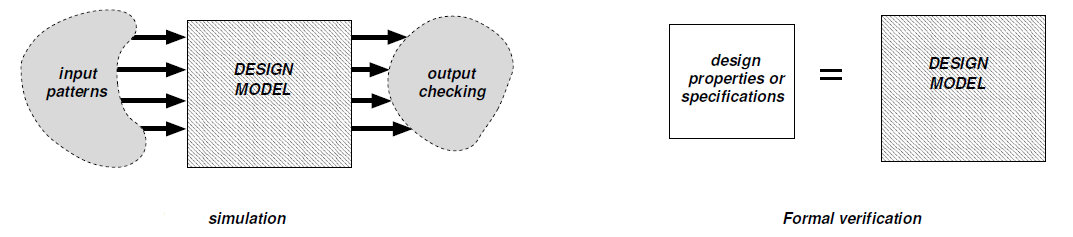
\includegraphics[width=\textwidth]{images/sim_vs_formal.PNG}
	\caption{On the right, a representation of the verification process by Simulation. Stimuli are applied to the DUV inputs and the output behaviour is checked. On the left, Formal Verification checks the DUV against a series of properties that describe the specified behaviour. \cite{thesis-formal}} \TLSAY{Good picture}
	\label{fig:sim-vs-formal}
\end{figure}

The idea of having mathematical proof of the soundness of a design, i.e. the implemented design corresponds to the specification, suggests complex work for the designer, or verification engineer. However, formal verification tools combine three main elements to provide the proof. It comprises proof methods, such as SAT-solving, some specific language, like propositional logic, and models, for example Finite State Machines (FSM). The designer must describe the system as a set of properties and provide them to the tool, which in turn will check if they hold for the RTL implementation. This formal method is also known as property checking. 

Property checking consists of heaving a set of properties describing the specified behaviour of the system and checking whether they can be proved, or checked, for the RTL design.  Therefore, it can be inferred that the RTL description design satisfies the specifications. 

The first step towards having a set of properties is to describe the specified design in an operational view, which can be divided into operations. Each operation represents a specific piece of functional behaviour in finite time interval of the DUV, and can be defined as follows:

\begin{itemize}
    \item Starting important state;
    \item Trigger condition;
    \item Ending important state;
    \item Output behaviour.
\end{itemize}

In other words, an operation describes the behaviour when the design is at a specific important state and a triggering condition happens. Then, the operation defines to which important state the design should go, as well the sequential output behaviour. 

Important states comprise the determination of values for the controls registers of the design. For this reason, they can be also referred as control states. Between the starting state and the ending state, the operation can pass through several non-important states that describe the data path of the design. The triggering condition usually refers to a sequence of inputs, but it can also be a control register having a specific value.

The idea of the operational view is to have a chain of operations that covers the full behaviour of the system. Thus, the end of an operation represents the beginning of other(s). In addition, parallel behaviour can be represented as parallel operations. Examples of operations for a design could be: a read or a write to memory or register file, waiting upon the arrival of a request signal, and the execution of an instruction in a processor.

After specifying the operational view of the design, each operation must be described as a property, or a set of properties, that capture its functionality. In practice, these properties can be written using, for example, System Verilog Assertion (SVA), Property Specification Language (PSL), or even commercial property languages such as ITL \cite{onespin}. A representation of a typical property cab be seen if Fig.~\ref{fig:property}.

\begin{figure}[htb!]
    \begin{lstlisting}
    property accept_request is
    assume:
        at t: state == S1;
        at t: request_i == 1;
    
    prove:
        at t+3: state == S2;
        at t+3: ack_o == 1;
    end property;
    \end{lstlisting}
    \caption{Example of a property that checks the behaviour for a request signal acknowledgement. At an arbitrary time $t$ the circuit is at state $S_1$ and a request signal arrives at the input port $request\_i$. At time $t+3$ the circuit should be at state $S_2$ and an acknowledgement signal is set at the output port $ack\_o$.}
    \label{fig:property}
\end{figure}

The two main parts of a property are the assumptions and commitments. The assumption part characterizes the starting important state and the triggering condition for the operation to be considered. The commitment part depicts the resulting behaviour if the operation is triggered, i.e. outputs description and ending state. A simplified way to represent a property is through a logical implication, Fig.~\ref{fig:a_impl_b}. If a set of assumptions are evaluated as $true$, then the commitments should also be evaluated as $true$ in order to make the property hold. An insight about how verification tools check operational properties is given on Sec.~\ref{subsection:ipc}. Before that, a brief introduction about finite state machines and SAT-solving is presented.

\begin{figure}[htb!]
    \begin{center}
        $a \longrightarrow b$
    \end{center}
    \caption{Logical implication operation where a implies b.}
    \label{fig:a_impl_b}
\end{figure}

\subsection*{Finite State Machine}

A Finite State Machine (FSM) is a deterministic and discrete model of computation that can be, among other applications, used to model a digital circuit. The definition of an FSM is given as follow:

\begin{itemize}
    \item[] $S$: a finite set of states;
    \item[] $s_{0}$: an initial state such that  $s_0 \in S$;
    \item[] $X$: a set of allowed input symbols, input alphabet;
    \item[] $Y$: a set of allowed output symbols, output alphabet;
    \item[] $\delta$: $S \times X \to S$ is a transition function;
    \item[] $\lambda$: $S \times Y \to Y$ is an output function.
\end{itemize}

There are two types of FSM, Mealy and Moore. The aforementioned definition refers to the Mealy type machine. The Moore type only differs on the output function which depends only on the current state $\lambda$: $S \to Y$.

Modelling an electrical circuit as an FSM means that each state of the state machine will correspond to a state of the circuit, i.e. a specific set of values for its control registers. A change of state, determined by the transaction function, and outputs, determined by the output function, will happen upon a change at the inputs. Fig.~\ref{fig:mealy_circuit} depicts a sequential circuit modelled from a Mealy machine.

\begin{figure}[htb!]
	\centering
	
\includegraphics[width=10cm]{images/mealy_circuit.png}
	\caption{Circuit model for a Mealy machine. The combinational circuit models the transition function $\delta$ and output function $\lambda$. The control registers model the state information.}
	\label{fig:mealy_circuit}
\end{figure}

\subsection*{SAT- Solving}

The propositional satisfiability problem, or simply SAT, is the problem of determining if a propositional formula, or Boolean expression, is $satisfiable$, i.e. if it can be evaluated as $true$ for some value combination for its variables. If there is no such combination, and the formula always evaluates to $false$, it is called $unsatisfiable$. 

Considering the formula in Fig.~\ref{fig:a_impl_b}, it is equivalent, and it can be converted, to the formula in the Fig.~\ref{fig:not_a_or_a_and_b}. This expression is $satisfiable$ because it evaluates to $true$ if $a$ is $false$ or if both $a$ and $b$ are $true$. This toy example illustrates how a general property could be converted into a Boolean expression and how SAT-solving could test its satisfiability.

\begin{figure}[htb!]
    \begin{center}
        $\neg a \lor a \land b$
    \end{center}
    \caption{Boolean expression equivalent to logical implication $a \longrightarrow b$.} \TLSAY{Why not not(a) or b ?} 
    \label{fig:not_a_or_a_and_b}
\end{figure}

\subsection{Interval Property Checking}
\label{subsection:ipc}

Interval Property Checking (IPC) is a formal method to prove an operational property for a design \TLINS{startign from a arbitrary time point ... and with an arbirtrary but fixed length}\TLDEL{at an arbitrary time interval}\TLSAY{Arbitrary time interval is wrong. The time interval is exactly given by time point and length}. Let us consider the sequential circuit in Fig.~\ref{fig:mealy_circuit} and a property that has its starting state at time $t$, and its ending state at time $t+3$, like the one in Fig.~\ref{fig:property}. The sequential circuit could be then converted into combinational by using the unrolling technique, Fig.~\ref{fig:unrolled}. The number of “unrolled circuits” will depend on the time interval of interest. In this case $[t, t+3]$.

\begin{figure}[htb!]
	\centering
	
\includegraphics[width=\textwidth]{images/unrolled_circuit.png}
	\caption{Unrolled circuit model for IPC. The unrolled circuit is converted into a Boolean expression which is used to check satisfiability.}
	\label{fig:unrolled}
\end{figure}

The variables from the “unrolled circuit” are then used to describe the property as a Boolean expression. Finally, the SAT-solving tool can evaluate whether the property is $satisfiable$ or not. In other words, IPC proves operational properties by constructing a combinational circuit for the design and solving a SAT problem for it. 

IPC is considered an unbounded model\TLSAY{not true} checking method because its time interval of interest can start at an arbitrary time point. It means that it does not start necessarily from the initial state of the circuit. The equivalent Boolean expression for the unbounded circuit from St to St+n is negated so that it cannot evaluate to $true$. If the SAT-solving tool finds a variable combination that evaluates the formula to $true$ it means that a failure was found. In other words, the property holds for the design if the expression is $unsatisfiable$ \TLSAY{dont use math env. for text just use textit}, otherwise, the respective variables combination that make the expression $satisfiable$ are presented by the tool as a counter-example.

Finding a counter-example does not necessarily means that there is a bug in the design. In fact, there could be a fault \TLSAY{its not a fault on the computational model ... it's just a spurious counter example} on the computational model. Since the starting state \TLREP{St}{$S_t$} can be arbitrary, it is important that it represents a reachable state of the design. During the verification process, when a property fails, the generated counter-example must be analysed in order to identify if it represents a possible scenario for the design of if it is a spurious counter-example, i.e. \TLREP{St}{$S_t$} \TLSAY{change everywhere} represents an unreachable state.

The reachability problem for IPC can be addressed by the concept of invariants. An invariant is a set of states that contains all states reachable from its own states. Let us consider for example a State Machine M. An invariant W of M is any set of states of M that contains all states reachable from W. In this sense, if a property holds for a state St E W, and W contains the initial state, the property holds for every reachable state of the system. Thus, if a spurious counter-example is generated by the tool, reachability information should be added to St as invariants. In practice, the assumptions of the property have to be constrained in order to represent a reachable state. 

\subsection{Gap-free verification}

As previously mentioned, the justification for using Formal Techniques to verify a digital design lies on its potential to achieve completeness \TLSAY{Completeness is not defined upon this point and its pretty special thing. You should express what completeness means in words upon the point of definition. Same is valid for gap-free. This also counts for your introduction}. In order to understand this concept better, let us first consider the notion of termination criteria. Conventional verification approaches have their termination criteria relying on the verification plan. Simulation based verification needs a verification plan that will result in a test bench that covers all possible \TLDEL{behaviour} scenario\TLINS{s}. This, of course, is very hard to \TLREP{achieve}{reach} for many designs even using random stimuli techniques. As for assertion-based verification (ABV), the hazard is on determining when the assertions written are enough to comprise the specified behaviour. Formal verification will have its termination criteria anchored on the concept of completeness.

A property set is said to be complete if it has a property, or subset of properties, describing each operation of a design, hence completely describing the specified behaviour of the system. With this, there is no gap between the RTL implementation and specifications, so the name \TLSAY{parse error} gap-free verification. \TLSAY{gap-free is a OneSpin trademark, you should reference their website}

\TLSAY{In text we imagine that a citation is the same as a person} \cite{paper-gapfree} defines a set of operation properties as complete, if it uniquely describes the output behaviour of a circuit according to determination requirements. These determination requirements specify which outputs and states variables are to be determined in each operation. To establish\TLSAY{wrong word ... check?} if a set of property is complete, the following completeness tests can be performed \cite{guide-onespin}:

\begin{enumerate}[A.]
    \item \textbf{The Case Split Test:} This test checks whether the chain of operations is comprised by the property set. Therefore, for each state reached by a property, there must be a property starting at this state for every input combination.
    \item \textbf{The Successor Test:} The successor test checks if the chain of properties is uniquely determined. In this sense, for every property the test check if each succeeding property is uniquely determined for its input trace.
    \item \textbf{The Determination Test:} This test will check the determination requirements. It verifies if the outputs and determined state registers, also referred as visible registers, are uniquely determined for all operations.
    \item \textbf{The Reset Property:} The reset test checks the initialization of the design. After the reset sequence, the design should end at a unique important state, and have determined all the signals according to the determination requirements.
\end{enumerate}


\section{Property-Driven Design}

\subsection{SystemC-PPA Model}

\subsubsection{PPA overview}

\subsubsection{SystemC-PPA}

\subsection{The PDD flow}

\subsection{DeSCAM}

\subsection{Completeness with S2QED}



\newpage
% ----------------------------------------------------------
% The Pipeline Algorithm
% ----------------------------------------------------------
\chapter{The Pipeline Algorithm}
\label{chapter:algorithm}

\section{PDD for Pipelined Processors}

\section{The Algorithm}

\section{The Plugin}

\textcolor{red}{Will this be a chapter or a section? Both algorithm plugin and s2qed skeleton plugin here?}
\newpage
% ----------------------------------------------------------
% The RI5cy Study Case
% ----------------------------------------------------------
\chapter{The RI5CY Study Case}

The algorithm to generate Pipeline Properties, proposed in Chap.~\ref{chapter:algorithm},  was evaluated with a case study for the RI5CY processor core. RI5CY is a 4-stage pipeline processor core based on the RISC-V architecture. Its implementation is open-source and powered by PULP Platform \cite{pulp}.

For this case study, a \textit{SystemC-PPA-compliant} \cite{paper-pdd} model for the chosen core was implemented as a sequential CPU. The properties were then automatically generated using DeSCAM \cite{descam}. From these automatically generated properties, the Pipeline Properties were finally created using the merging Pipeline Algorithm. 

This chapter starts with a brief discussion about the RISC-V Implementation Set Architecture in Sec.~\ref{section:riscv} and the RI5CY processor core in Sec.~\ref{section:ri5cy_core}. Next, the ESL implementation compliant to the \textit{SystemC-PPA} specification is detailed in Sec.~\ref{section:ri5cy_esl}. Then, the DeSCAM generated properties are presented in Sec.~\ref{section:ri5cy_micro_ppt}, followed by the Pipeline Properties in Sec.~\ref{section:ri5cy_pipe_ppt}, and finally the S2QED Properties Sec.~\ref{section:ri5cy_s2qed_ppt}.

\section{RIVC-V ISA Overview}
\label{section:riscv}
Instruction Set Architecture (ISA), as the name suggests, is the set of instructions that a computer, or more specifically a processor core, can execute. Among other things, an ISA specification will determine which operations the processor can perform, how the memory is addressed and the type and size of the instruction operands \cite{book-comp-arch}.

A Reduced Instruction Set Computer (RISC) is a computer that has a small set of instructions. These instructions have a simple fixed length encoding, and they take similar number of \textit{clock} cycles to execute \cite{book-comp-arch}. Some examples of RISC architectures are AMRv7, MIPS and RISC-V.

RISC-V is an open ISA that offers both a small base integer ISA that can be used by itself, and optional standard extensions. As an open and free to use architecture, it was initially intended to support computer architecture research and education \cite{spec-riscv}. Even so, its popularity increased rapidly and there are open-source simulators, compilers, debuggers and implementations in Hardware Description Language (HDL) for RISC-V available \cite{book-comp-org}. One of these open-source implementations is the RI5CY processor powered by PULP Platform \cite{pulp}. This implementation is used as case study in the present work and some important details are presented in the next section. 

\section{The RI5CY Processor Core}
\label{section:ri5cy_core}

RI5CY is a processor core implementation based on the RISC-V ISA. It is an in-order \textit{32 bits} core and has a pipeline with 4 stages. Besides the support for the \textit{RV32I} Base Integer Instruction Set, it has also support for the \textit{RV32C} Standard Extension for Compressed Instructions and \textit{RV32M} Integer Multiplication and Division Instruction Set Extension, and optional support for \textit{RV32F} Single Precision Floating Point Extensions. This core also implements the following PUPL specific extensions:  Post-Incrementing load and stores, Multiply-Accumulate extensions, ALU extensions, and Hardware Loops.

However, this case study is focused on the \textit{32bits} Integer Base Instructions set \textcolor{red}{[maybe some standard extensions if time allows it]} as detailed in Sec.~\ref{section:ri5cy_esl} of this chapter. Before that, however, some aspects of the pipeline, memory protocol and Load-Store Unit of the RI5CY core are briefely discussed. These implementation aspects are important for the understanding of the ESL model and for the property generation as well.

For detailed information about all the RI5CY implemented extensions, the reader can refer to the RI5CY User Manual \cite{manual-ri5cy}.

\subsection*{RI5CY Pipeline}

As aforementioned, this core implements a 4-stages pipeline: instruction fetch ($IF$), instruction decode ($ID$), execute ($EX$) and write-back ($WB$). However, most of the instructions in the base integer set, like arithmetic and logic operations, uses only the first three stages. The $WB$ stage is used, for example, when loading data from the data memory. Fig.~\ref{fig:ri5cy_pipeline} depicts the pipeline structure and its main signals.

\begin{figure}[htb!]
	\centering
	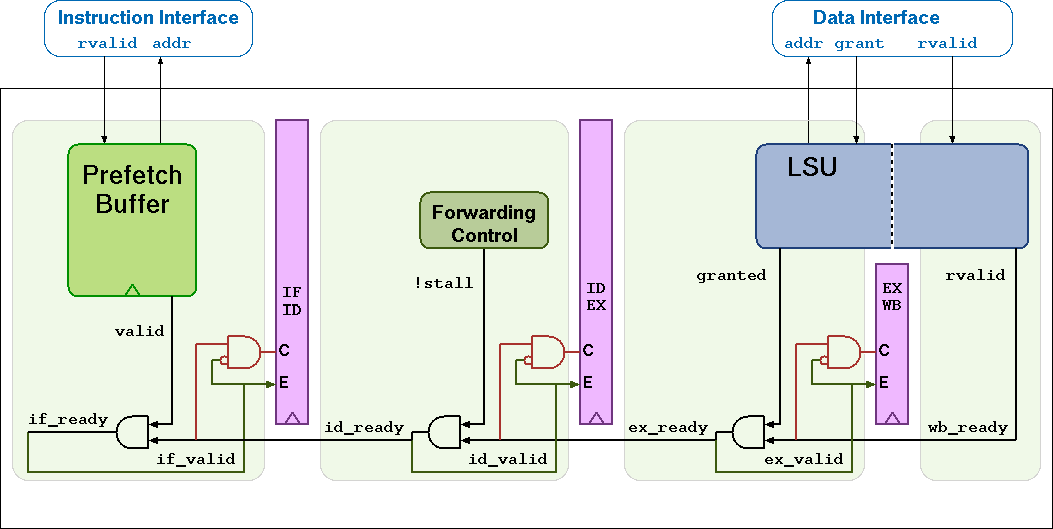
\includegraphics[width=\textwidth]{images/ri5cy_pipeline.png}
	\caption{RI5CY pipeline diagram \cite{manual-ri5cy}.}
	\label{fig:ri5cy_pipeline}
\end{figure}

The ready signal of each stage propagates from right to left and are used to inform the previous stage that the current stage is ready to operate. In this sense, each stage can finish its execution independently from the previous, but they cannot propagate (stall) if the next one is not ready. 

\subsection*{RI5CY Load-Store Unit}

The Load-Store Unit (LSU) is the component of the core responsible to access the data memory. As shown in Fig.~\ref{fig:ri5cy_pipeline}, the LSU belongs to two pipeline stages: $EX$ and $WB$. It means that a request to the data memory is sent already in the $EX$ stage. To illustrate this behaviour better, consider a LOAD instruction in the ID stage. In the next \textit{clock} cycle, the access address is computed in the $EX$ stage, and the LSU sends a request to the data memory in the same cycle. When the data arrives from memory, the LSU will write it to the correspondent register in the $WB$ stage. The memory access protocol is detailed next.

\subsection*{RI5CY Memory Access Protocol}

In order to access the data memory, the LSU sets the output address with the right address and sends a request signal. The LSU waits for a grant signal from the memory that can come in the same \textit{clock} cycle as the request or any number of \textit{clock} cycles later. After receiving the grant signal, the LSU can optionally change the outputs and make a new request or just set the request signal to low. If it was a read from memory request, e.g. LOAD instruction, the memory will send the data along with a valid signal one or more \textit{clock} cycles after the grant signal. All the LSU signals can be found on Table~\ref{tab:lsu-signals} with a brief description. 

\begin{table*}[htb!] 
	\centering 
	\caption{LSU port signals of RI5CY processor\cite{manual-ri5cy}.} 
	\label{tab:lsu-signals}
	\begin{tabular}{l|c|p{7cm}} 
		\multicolumn{1}{c}{\bfseries Signal} & \multicolumn{1}{c}{\bfseries Port Direction} & \multicolumn{1}{c}{\bfseries Description} \\     
		\hline	
		$data\_req\_o$  &  output & Request ready, must stay high until $data\_gnt\_i$ is        high for one cycle \\
		\hline
		$data\_addr\_o$[31:0]  &  output & Address \\
		\hline
		$data\_we\_o$  &  output & Write Enable, high for writes, low for reads. Sent            together with $data\_req\_o$ \\
		\hline
		$data\_wdata\_o$[31:0]  &  output & Data to be written to memory, sent together with     $data\_req\_o$ \\
		\hline
		$data\_rdata\_i$[31:0]  &  input & Data read from memory \\
		\hline
		$data\_rvalid\_i$  &  input & $data\_rdata\_i$ holds valid data when                     $data\_rvalid\_i$ is high. This signal will be high for exactly one cycle per        request. \\
		\hline
		$data\_gnt\_i$  &  input & The other side accepted the request. $data\_addr\_o$ may     change in the next cycle \\
		\hline
	\end{tabular} 
\end{table*}

The instruction memory access performed by the instruction fetcher of the core is similar to the data memory protocol. The only difference is that that the instruction fetcher does not have any writing interface, since the instruction memory is only read by the core. The instruction fetcher signals are presented on Table~\ref{tab:imem-signals}.

\begin{table*}[htb!] 
	\centering 
	\caption{Instruction memory port signals of RI5CY processor \cite{manual-ri5cy}.} 
	\label{tab:imem-signals}
	\begin{tabular}{l|c|p{7cm}} 
		\multicolumn{1}{c}{\bfseries Signal} & \multicolumn{1}{c}{\bfseries Port Direction} & \multicolumn{1}{c}{\bfseries Description} \\     
		\hline	
		$instr\_req\_o$  &  output & Request ready, must stay high until $instr\_gnt\_i$ is high for one cycle \\
		\hline
		$instr\_addr\_o$[31:0]  &  output & Address \\
		\hline
		$instr\_rdata\_i$[31:0]  &  input & Data read from memory \\
		\hline
		$instr\_rvalid\_i$  &  input & $instr\_rdata\_i$ holds valid data when $instr\_rvalid\_i$ is high. This signal will be high for exactly one cycle per request. \\
		\hline
		$instr\_gnt\_i$  &  input & The other side accepted the request. $instr\_addr\_o$ may change in the next cycle \\
		\hline
	\end{tabular} 
\end{table*}

\section{RI5CY ESL Implementation}
\label{section:ri5cy_esl}

\section{The DeSCAM Properties}
\label{section:ri5cy_micro_ppt}

\section{The Pipeline Properties}
\label{section:ri5cy_pipe_ppt}

\section{The S2QED Properties}
\label{section:ri5cy_s2qed_ppt}
\newpage
% ----------------------------------------------------------
% Results
% ----------------------------------------------------------
\chapter{Results}
\newpage
% ----------------------------------------------------------
% Conclusion
% ----------------------------------------------------------
\chapter{Conclusion}
\newpage
% \input{chapters/6_ausblick.tex}
% \newpage

\backmatter
\listoffigures 
\listoftables
% \listoflistings

%%%%%%%%%%%%%%%%%%%%%%%%%%%%%%%%%%%%%%%%%%%%%%%%%%%%%%%%%%%%%%%%%%%%%%%%
% Choose your Bibtex Style File (here alphadin.bst) and references.
% Hint: For references make a local link refs2 to our jabref 
% directory "/import/jabref/refs2.bib"
%%%%%%%%%%%%%%%%%%%%%%%%%%%%%%%%%%%%%%%%%%%%%%%%%%%%%%%%%%%%%%%%%%%%%%%%

%%%%%%%%%%%%%%%%%%%%%%%%%%%%%%%%%%%%%%%%%%%%%%%%%%%%%%%%%%%%%%%%%%%%%%%%
% \bibliographystyle{alphadin}
\bibliographystyle{plain}
% \bibliography{refs3}
\bibliography{myrefs} %I added this
% \bibliography{myrefs}
% \input{mybiblio}%\todo{use bibtex!}
%%%%%%%%%%%%%%%%%%%%%%%%%%%%%%%%%%%%%%%%%%%%%%%%%%%%%%%%%%%%%%%%%%%%%%%%

%%%%%%%%%%%%%%%%%%%%%%%%%%%%%%%%%%%%%%%%%%%%%%%%%%%%%%%%%%%%%%%%%%%%%%%%
% Curriculum Vitae
%%%%%%%%%%%%%%%%%%%%%%%%%%%%%%%%%%%%%%%%%%%%%%%%%%%%%%%%%%%%%%%%%%%%%%%%
%\selectlanguage{german}
%\input{cv.tex}
%\selectlanguage{english}

\end{document}
